\documentclass[twoside]{book}

% Packages required by doxygen
\usepackage{fixltx2e}
\usepackage{calc}
\usepackage{doxygen}
\usepackage[export]{adjustbox} % also loads graphicx
\usepackage{graphicx}
\usepackage[utf8]{inputenc}
\usepackage{makeidx}
\usepackage{multicol}
\usepackage{multirow}
\PassOptionsToPackage{warn}{textcomp}
\usepackage{textcomp}
\usepackage[nointegrals]{wasysym}
\usepackage[table]{xcolor}

% Font selection
\usepackage[T1]{fontenc}
\usepackage[scaled=.90]{helvet}
\usepackage{courier}
\usepackage{amssymb}
\usepackage{sectsty}
\renewcommand{\familydefault}{\sfdefault}
\allsectionsfont{%
  \fontseries{bc}\selectfont%
  \color{darkgray}%
}
\renewcommand{\DoxyLabelFont}{%
  \fontseries{bc}\selectfont%
  \color{darkgray}%
}
\newcommand{\+}{\discretionary{\mbox{\scriptsize$\hookleftarrow$}}{}{}}

% Page & text layout
\usepackage{geometry}
\geometry{%
  a4paper,%
  top=2.5cm,%
  bottom=2.5cm,%
  left=2.5cm,%
  right=2.5cm%
}
\tolerance=750
\hfuzz=15pt
\hbadness=750
\setlength{\emergencystretch}{15pt}
\setlength{\parindent}{0cm}
\setlength{\parskip}{3ex plus 2ex minus 2ex}
\makeatletter
\renewcommand{\paragraph}{%
  \@startsection{paragraph}{4}{0ex}{-1.0ex}{1.0ex}{%
    \normalfont\normalsize\bfseries\SS@parafont%
  }%
}
\renewcommand{\subparagraph}{%
  \@startsection{subparagraph}{5}{0ex}{-1.0ex}{1.0ex}{%
    \normalfont\normalsize\bfseries\SS@subparafont%
  }%
}
\makeatother

% Headers & footers
\usepackage{fancyhdr}
\pagestyle{fancyplain}
\fancyhead[LE]{\fancyplain{}{\bfseries\thepage}}
\fancyhead[CE]{\fancyplain{}{}}
\fancyhead[RE]{\fancyplain{}{\bfseries\leftmark}}
\fancyhead[LO]{\fancyplain{}{\bfseries\rightmark}}
\fancyhead[CO]{\fancyplain{}{}}
\fancyhead[RO]{\fancyplain{}{\bfseries\thepage}}
\fancyfoot[LE]{\fancyplain{}{}}
\fancyfoot[CE]{\fancyplain{}{}}
\fancyfoot[RE]{\fancyplain{}{\bfseries\scriptsize Generated by Doxygen }}
\fancyfoot[LO]{\fancyplain{}{\bfseries\scriptsize Generated by Doxygen }}
\fancyfoot[CO]{\fancyplain{}{}}
\fancyfoot[RO]{\fancyplain{}{}}
\renewcommand{\footrulewidth}{0.4pt}
\renewcommand{\chaptermark}[1]{%
  \markboth{#1}{}%
}
\renewcommand{\sectionmark}[1]{%
  \markright{\thesection\ #1}%
}

% Indices & bibliography
\usepackage{natbib}
\usepackage[titles]{tocloft}
\setcounter{tocdepth}{3}
\setcounter{secnumdepth}{5}
\makeindex

% Hyperlinks (required, but should be loaded last)
\usepackage{ifpdf}
\ifpdf
  \usepackage[pdftex,pagebackref=true]{hyperref}
\else
  \usepackage[ps2pdf,pagebackref=true]{hyperref}
\fi
\hypersetup{%
  colorlinks=true,%
  linkcolor=blue,%
  citecolor=blue,%
  unicode%
}

% Custom commands
\newcommand{\clearemptydoublepage}{%
  \newpage{\pagestyle{empty}\cleardoublepage}%
}

\usepackage{caption}
\captionsetup{labelsep=space,justification=centering,font={bf},singlelinecheck=off,skip=4pt,position=top}

%===== C O N T E N T S =====

\begin{document}

% Titlepage & ToC
\hypersetup{pageanchor=false,
             bookmarksnumbered=true,
             pdfencoding=unicode
            }
\pagenumbering{alph}
\begin{titlepage}
\vspace*{7cm}
\begin{center}%
{\Large My Project }\\
\vspace*{1cm}
{\large Generated by Doxygen 1.8.13}\\
\end{center}
\end{titlepage}
\clearemptydoublepage
\pagenumbering{roman}
\tableofcontents
\clearemptydoublepage
\pagenumbering{arabic}
\hypersetup{pageanchor=true}

%--- Begin generated contents ---
\chapter{Hierarchical Index}
\section{Class Hierarchy}
This inheritance list is sorted roughly, but not completely, alphabetically\+:\begin{DoxyCompactList}
\item \contentsline{section}{test.\+Bishop\+Test}{\pageref{classtest_1_1_bishop_test}}{}
\item \contentsline{section}{main.\+Board}{\pageref{classmain_1_1_board}}{}
\begin{DoxyCompactList}
\item \contentsline{section}{main.\+Check}{\pageref{classmain_1_1_check}}{}
\end{DoxyCompactList}
\item \contentsline{section}{test.\+Board\+Test}{\pageref{classtest_1_1_board_test}}{}
\item \contentsline{section}{test.\+Check\+Test}{\pageref{classtest_1_1_check_test}}{}
\item \contentsline{section}{G\+U\+I.\+Game}{\pageref{class_g_u_i_1_1_game}}{}
\item \contentsline{section}{test.\+King\+Test}{\pageref{classtest_1_1_king_test}}{}
\item \contentsline{section}{test.\+Knight\+Test}{\pageref{classtest_1_1_knight_test}}{}
\item \contentsline{section}{Main}{\pageref{class_main}}{}
\item \contentsline{section}{test.\+Pawn\+Test}{\pageref{classtest_1_1_pawn_test}}{}
\item \contentsline{section}{main.\+Piece}{\pageref{classmain_1_1_piece}}{}
\begin{DoxyCompactList}
\item \contentsline{section}{main.\+Bishop}{\pageref{classmain_1_1_bishop}}{}
\item \contentsline{section}{main.\+King}{\pageref{classmain_1_1_king}}{}
\item \contentsline{section}{main.\+Knight}{\pageref{classmain_1_1_knight}}{}
\item \contentsline{section}{main.\+Pawn}{\pageref{classmain_1_1_pawn}}{}
\item \contentsline{section}{main.\+Queen}{\pageref{classmain_1_1_queen}}{}
\item \contentsline{section}{main.\+Rook}{\pageref{classmain_1_1_rook}}{}
\item \contentsline{section}{main.\+Special\+Beep}{\pageref{classmain_1_1_special_beep}}{}
\item \contentsline{section}{main.\+Special\+Boop}{\pageref{classmain_1_1_special_boop}}{}
\end{DoxyCompactList}
\item \contentsline{section}{main.\+Position}{\pageref{classmain_1_1_position}}{}
\item \contentsline{section}{test.\+Queen\+Test}{\pageref{classtest_1_1_queen_test}}{}
\item \contentsline{section}{test.\+Rook\+Test}{\pageref{classtest_1_1_rook_test}}{}
\end{DoxyCompactList}

\chapter{Class Index}
\section{Class List}
Here are the classes, structs, unions and interfaces with brief descriptions\+:\begin{DoxyCompactList}
\item\contentsline{section}{\hyperlink{classmain_1_1_bishop}{main.\+Bishop} }{\pageref{classmain_1_1_bishop}}{}
\item\contentsline{section}{\hyperlink{classtest_1_1_bishop_test}{test.\+Bishop\+Test} }{\pageref{classtest_1_1_bishop_test}}{}
\item\contentsline{section}{\hyperlink{classmain_1_1_board}{main.\+Board} }{\pageref{classmain_1_1_board}}{}
\item\contentsline{section}{\hyperlink{classtest_1_1_board_test}{test.\+Board\+Test} }{\pageref{classtest_1_1_board_test}}{}
\item\contentsline{section}{\hyperlink{classmain_1_1_check}{main.\+Check} }{\pageref{classmain_1_1_check}}{}
\item\contentsline{section}{\hyperlink{classtest_1_1_check_test}{test.\+Check\+Test} }{\pageref{classtest_1_1_check_test}}{}
\item\contentsline{section}{\hyperlink{class_g_u_i_1_1_game}{G\+U\+I.\+Game} }{\pageref{class_g_u_i_1_1_game}}{}
\item\contentsline{section}{\hyperlink{classmain_1_1_king}{main.\+King} }{\pageref{classmain_1_1_king}}{}
\item\contentsline{section}{\hyperlink{classtest_1_1_king_test}{test.\+King\+Test} }{\pageref{classtest_1_1_king_test}}{}
\item\contentsline{section}{\hyperlink{classmain_1_1_knight}{main.\+Knight} }{\pageref{classmain_1_1_knight}}{}
\item\contentsline{section}{\hyperlink{classtest_1_1_knight_test}{test.\+Knight\+Test} }{\pageref{classtest_1_1_knight_test}}{}
\item\contentsline{section}{\hyperlink{class_main}{Main} }{\pageref{class_main}}{}
\item\contentsline{section}{\hyperlink{classmain_1_1_pawn}{main.\+Pawn} }{\pageref{classmain_1_1_pawn}}{}
\item\contentsline{section}{\hyperlink{classtest_1_1_pawn_test}{test.\+Pawn\+Test} }{\pageref{classtest_1_1_pawn_test}}{}
\item\contentsline{section}{\hyperlink{classmain_1_1_piece}{main.\+Piece} }{\pageref{classmain_1_1_piece}}{}
\item\contentsline{section}{\hyperlink{classmain_1_1_position}{main.\+Position} }{\pageref{classmain_1_1_position}}{}
\item\contentsline{section}{\hyperlink{classmain_1_1_queen}{main.\+Queen} }{\pageref{classmain_1_1_queen}}{}
\item\contentsline{section}{\hyperlink{classtest_1_1_queen_test}{test.\+Queen\+Test} }{\pageref{classtest_1_1_queen_test}}{}
\item\contentsline{section}{\hyperlink{classmain_1_1_rook}{main.\+Rook} }{\pageref{classmain_1_1_rook}}{}
\item\contentsline{section}{\hyperlink{classtest_1_1_rook_test}{test.\+Rook\+Test} }{\pageref{classtest_1_1_rook_test}}{}
\item\contentsline{section}{\hyperlink{classmain_1_1_special_beep}{main.\+Special\+Beep} }{\pageref{classmain_1_1_special_beep}}{}
\item\contentsline{section}{\hyperlink{classmain_1_1_special_boop}{main.\+Special\+Boop} }{\pageref{classmain_1_1_special_boop}}{}
\end{DoxyCompactList}

\chapter{Class Documentation}
\hypertarget{classmain_1_1_bishop}{}\section{main.\+Bishop Class Reference}
\label{classmain_1_1_bishop}\index{main.\+Bishop@{main.\+Bishop}}
Inheritance diagram for main.\+Bishop\+:\begin{figure}[H]
\begin{center}
\leavevmode
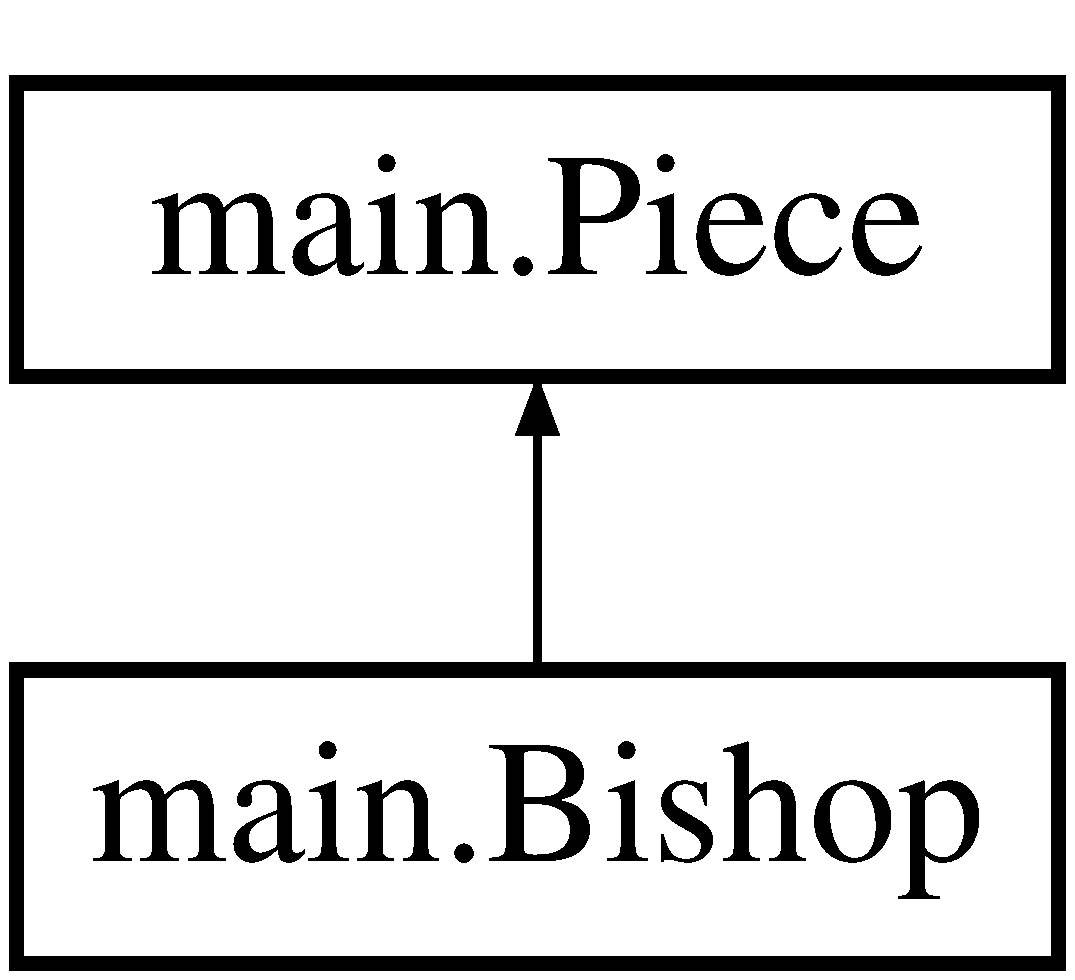
\includegraphics[height=2.000000cm]{classmain_1_1_bishop}
\end{center}
\end{figure}
\subsection*{Public Member Functions}
\begin{DoxyCompactItemize}
\item 
\hyperlink{classmain_1_1_bishop_ae4a17c8ad184c8f0240c7c2c29f52b38}{Bishop} (int player, \hyperlink{classmain_1_1_position}{Position} position, \hyperlink{classmain_1_1_board}{Board} board)
\item 
boolean \hyperlink{classmain_1_1_bishop_ac7443304a05994dba25f2a53fe83e452}{can\+Move\+To} (int x, int y)
\end{DoxyCompactItemize}


\subsection{Constructor \& Destructor Documentation}
\mbox{\Hypertarget{classmain_1_1_bishop_ae4a17c8ad184c8f0240c7c2c29f52b38}\label{classmain_1_1_bishop_ae4a17c8ad184c8f0240c7c2c29f52b38}} 
\index{main\+::\+Bishop@{main\+::\+Bishop}!Bishop@{Bishop}}
\index{Bishop@{Bishop}!main\+::\+Bishop@{main\+::\+Bishop}}
\subsubsection{\texorpdfstring{Bishop()}{Bishop()}}
{\footnotesize\ttfamily main.\+Bishop.\+Bishop (\begin{DoxyParamCaption}\item[{int}]{player,  }\item[{\hyperlink{classmain_1_1_position}{Position}}]{position,  }\item[{\hyperlink{classmain_1_1_board}{Board}}]{board }\end{DoxyParamCaption})}

Constructor for the \hyperlink{classmain_1_1_bishop}{Bishop} class 
\begin{DoxyParams}{Parameters}
{\em player} & piece player/owner \\
\hline
{\em position} & location of the piece on the board \\
\hline
{\em board} & game board \\
\hline
\end{DoxyParams}


\subsection{Member Function Documentation}
\mbox{\Hypertarget{classmain_1_1_bishop_ac7443304a05994dba25f2a53fe83e452}\label{classmain_1_1_bishop_ac7443304a05994dba25f2a53fe83e452}} 
\index{main\+::\+Bishop@{main\+::\+Bishop}!can\+Move\+To@{can\+Move\+To}}
\index{can\+Move\+To@{can\+Move\+To}!main\+::\+Bishop@{main\+::\+Bishop}}
\subsubsection{\texorpdfstring{can\+Move\+To()}{canMoveTo()}}
{\footnotesize\ttfamily boolean main.\+Bishop.\+can\+Move\+To (\begin{DoxyParamCaption}\item[{int}]{x,  }\item[{int}]{y }\end{DoxyParamCaption})}

Function for checking if the piece can move to a specified (x,y) position on the board 
\begin{DoxyParams}{Parameters}
{\em x} & position along the x axis \\
\hline
{\em y} & position along the y axis \\
\hline
\end{DoxyParams}
\begin{DoxyReturn}{Returns}
true/false boolean whether it\textquotesingle{}s a valid move 
\end{DoxyReturn}


The documentation for this class was generated from the following file\+:\begin{DoxyCompactItemize}
\item 
src/main/Bishop.\+java\end{DoxyCompactItemize}

\hypertarget{classtest_1_1_bishop_test}{}\section{test.\+Bishop\+Test Class Reference}
\label{classtest_1_1_bishop_test}\index{test.\+Bishop\+Test@{test.\+Bishop\+Test}}
\subsection*{Public Member Functions}
\begin{DoxyCompactItemize}
\item 
\mbox{\Hypertarget{classtest_1_1_bishop_test_a17eecddbdfc11bde69d27d5ef42462c6}\label{classtest_1_1_bishop_test_a17eecddbdfc11bde69d27d5ef42462c6}} 
void {\bfseries test\+Position} ()  throws Exception 
\item 
\mbox{\Hypertarget{classtest_1_1_bishop_test_a29cbfa954c25992b79e8838c987eafb3}\label{classtest_1_1_bishop_test_a29cbfa954c25992b79e8838c987eafb3}} 
void {\bfseries test\+Valid\+Move} ()  throws Exception 
\item 
\mbox{\Hypertarget{classtest_1_1_bishop_test_a8fdf33a4359a7403b6a43810326da7ae}\label{classtest_1_1_bishop_test_a8fdf33a4359a7403b6a43810326da7ae}} 
void {\bfseries test\+Invalid\+Move} ()  throws Exception 
\end{DoxyCompactItemize}


The documentation for this class was generated from the following file\+:\begin{DoxyCompactItemize}
\item 
src/test/Bishop\+Test.\+java\end{DoxyCompactItemize}

\hypertarget{classmain_1_1_board}{}\section{main.\+Board Class Reference}
\label{classmain_1_1_board}\index{main.\+Board@{main.\+Board}}
Inheritance diagram for main.\+Board\+:\begin{figure}[H]
\begin{center}
\leavevmode
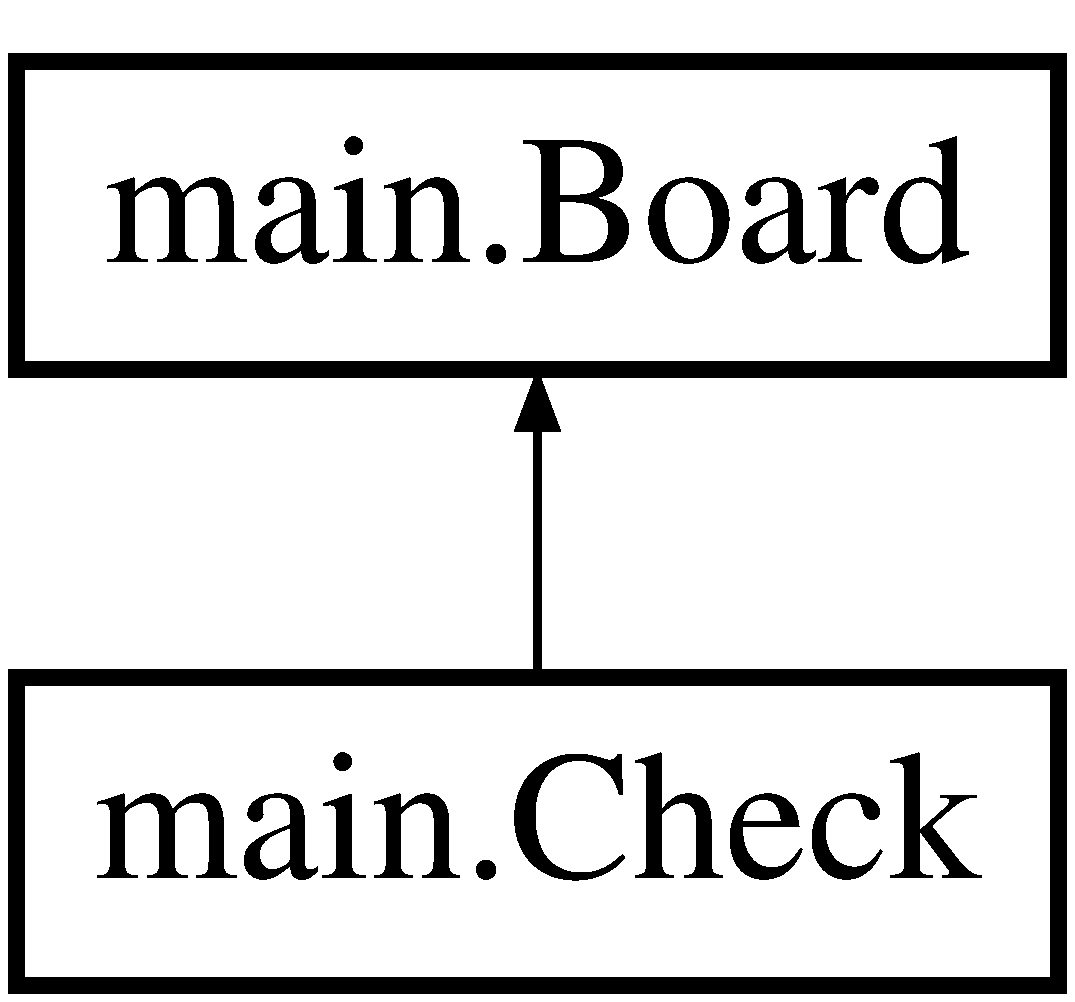
\includegraphics[height=2.000000cm]{classmain_1_1_board}
\end{center}
\end{figure}
\subsection*{Public Member Functions}
\begin{DoxyCompactItemize}
\item 
\hyperlink{classmain_1_1_board_ac64a3f3f09655e7a7c8d357571a0cdf9}{Board} ()
\item 
int \hyperlink{classmain_1_1_board_aabe840fa797394de39d654669f1a13e3}{get\+Row\+Size} ()
\item 
int \hyperlink{classmain_1_1_board_ad54aaad9c4592f90902c9176178479f4}{get\+Col\+Size} ()
\item 
\hyperlink{classmain_1_1_piece}{Piece} \hyperlink{classmain_1_1_board_ab7453028b7be41317754865bd98e7c27}{get\+Piece} (int x, int y)
\item 
\mbox{\Hypertarget{classmain_1_1_board_a3251505af2aca3cba6f42d187c2dedd5}\label{classmain_1_1_board_a3251505af2aca3cba6f42d187c2dedd5}} 
\hyperlink{classmain_1_1_piece}{Piece} \mbox{[}$\,$\mbox{]}\mbox{[}$\,$\mbox{]} {\bfseries get\+Board} ()
\item 
void \hyperlink{classmain_1_1_board_ae50e0afff7effa41b09eb9966983e369}{add\+Piece} (\hyperlink{classmain_1_1_piece}{Piece} piece)
\item 
void \hyperlink{classmain_1_1_board_a3a4955259c7cf7ad67524f8da986d23b}{move\+Piece} (\hyperlink{classmain_1_1_piece}{Piece} piece, \hyperlink{classmain_1_1_position}{Position} p)
\item 
void \hyperlink{classmain_1_1_board_abc2d60f853b5da298d709637546758f8}{remove\+Piece} (\hyperlink{classmain_1_1_piece}{Piece} piece)
\item 
boolean \hyperlink{classmain_1_1_board_a13d0c13bb4ac27d6f7f6c7695eb2fb3e}{check\+Diagonal\+Move} (\hyperlink{classmain_1_1_piece}{Piece} piece, int x, int y)
\item 
\mbox{\Hypertarget{classmain_1_1_board_afc7aebf0d29dce28ea6b358cc77f8638}\label{classmain_1_1_board_afc7aebf0d29dce28ea6b358cc77f8638}} 
boolean {\bfseries check\+In\+Line\+Move\+Helper} (int curra, int currb, int a, int b)
\item 
boolean \hyperlink{classmain_1_1_board_a41d11b3b542eaa65607bc50c0a8ab6b4}{check\+In\+Line\+Move} (\hyperlink{classmain_1_1_piece}{Piece} piece, int x, int y)
\item 
\mbox{\Hypertarget{classmain_1_1_board_a5e439108a532952162da1d08560dd260}\label{classmain_1_1_board_a5e439108a532952162da1d08560dd260}} 
void {\bfseries set\+Pawns} (\hyperlink{classmain_1_1_board}{Board} board, boolean custom)
\item 
\mbox{\Hypertarget{classmain_1_1_board_a3295974eeb0e6fe02673aaf43a6c2709}\label{classmain_1_1_board_a3295974eeb0e6fe02673aaf43a6c2709}} 
void {\bfseries set\+Bishops} (\hyperlink{classmain_1_1_board}{Board} board)
\item 
\mbox{\Hypertarget{classmain_1_1_board_a3f25d1c4cf5a1140b7b3e38d9a50b737}\label{classmain_1_1_board_a3f25d1c4cf5a1140b7b3e38d9a50b737}} 
void {\bfseries set\+Kings} (\hyperlink{classmain_1_1_board}{Board} board)
\item 
\mbox{\Hypertarget{classmain_1_1_board_ae8f371f340211e79784f066eeea57053}\label{classmain_1_1_board_ae8f371f340211e79784f066eeea57053}} 
void {\bfseries set\+Knights} (\hyperlink{classmain_1_1_board}{Board} board)
\item 
\mbox{\Hypertarget{classmain_1_1_board_a74ea62c7573eaf06b0d59ea9f258184b}\label{classmain_1_1_board_a74ea62c7573eaf06b0d59ea9f258184b}} 
void {\bfseries set\+Queens} (\hyperlink{classmain_1_1_board}{Board} board)
\item 
\mbox{\Hypertarget{classmain_1_1_board_a56f872c4ad1d69c733e6c31662f1af1f}\label{classmain_1_1_board_a56f872c4ad1d69c733e6c31662f1af1f}} 
void {\bfseries set\+Rooks} (\hyperlink{classmain_1_1_board}{Board} board)
\item 
void \hyperlink{classmain_1_1_board_abc9e551a462c7fec722d11e5f3728c23}{init\+Pieces} (\hyperlink{classmain_1_1_board}{Board} board, boolean custom)
\end{DoxyCompactItemize}


\subsection{Constructor \& Destructor Documentation}
\mbox{\Hypertarget{classmain_1_1_board_ac64a3f3f09655e7a7c8d357571a0cdf9}\label{classmain_1_1_board_ac64a3f3f09655e7a7c8d357571a0cdf9}} 
\index{main\+::\+Board@{main\+::\+Board}!Board@{Board}}
\index{Board@{Board}!main\+::\+Board@{main\+::\+Board}}
\subsubsection{\texorpdfstring{Board()}{Board()}}
{\footnotesize\ttfamily main.\+Board.\+Board (\begin{DoxyParamCaption}{ }\end{DoxyParamCaption})}

Constructor for the game board, initializes all position on the board to null 

\subsection{Member Function Documentation}
\mbox{\Hypertarget{classmain_1_1_board_ae50e0afff7effa41b09eb9966983e369}\label{classmain_1_1_board_ae50e0afff7effa41b09eb9966983e369}} 
\index{main\+::\+Board@{main\+::\+Board}!add\+Piece@{add\+Piece}}
\index{add\+Piece@{add\+Piece}!main\+::\+Board@{main\+::\+Board}}
\subsubsection{\texorpdfstring{add\+Piece()}{addPiece()}}
{\footnotesize\ttfamily void main.\+Board.\+add\+Piece (\begin{DoxyParamCaption}\item[{\hyperlink{classmain_1_1_piece}{Piece}}]{piece }\end{DoxyParamCaption})}

Function that initializes a piece in its position 
\begin{DoxyParams}{Parameters}
{\em piece} & the desired piece to position \\
\hline
\end{DoxyParams}
\mbox{\Hypertarget{classmain_1_1_board_a13d0c13bb4ac27d6f7f6c7695eb2fb3e}\label{classmain_1_1_board_a13d0c13bb4ac27d6f7f6c7695eb2fb3e}} 
\index{main\+::\+Board@{main\+::\+Board}!check\+Diagonal\+Move@{check\+Diagonal\+Move}}
\index{check\+Diagonal\+Move@{check\+Diagonal\+Move}!main\+::\+Board@{main\+::\+Board}}
\subsubsection{\texorpdfstring{check\+Diagonal\+Move()}{checkDiagonalMove()}}
{\footnotesize\ttfamily boolean main.\+Board.\+check\+Diagonal\+Move (\begin{DoxyParamCaption}\item[{\hyperlink{classmain_1_1_piece}{Piece}}]{piece,  }\item[{int}]{x,  }\item[{int}]{y }\end{DoxyParamCaption})}

Function that checks if a diagonal move of a position is valid by checking all positions along the diagonal and seeing if there is any other pieces on the board 
\begin{DoxyParams}{Parameters}
{\em piece} & the piece to check the diagonal from \\
\hline
{\em x} & the position on the x axis of the desired new position \\
\hline
{\em y} & the position on the y axis of the desired new position \\
\hline
\end{DoxyParams}
\begin{DoxyReturn}{Returns}
true/false boolean whether the move is valid 
\end{DoxyReturn}
\mbox{\Hypertarget{classmain_1_1_board_a41d11b3b542eaa65607bc50c0a8ab6b4}\label{classmain_1_1_board_a41d11b3b542eaa65607bc50c0a8ab6b4}} 
\index{main\+::\+Board@{main\+::\+Board}!check\+In\+Line\+Move@{check\+In\+Line\+Move}}
\index{check\+In\+Line\+Move@{check\+In\+Line\+Move}!main\+::\+Board@{main\+::\+Board}}
\subsubsection{\texorpdfstring{check\+In\+Line\+Move()}{checkInLineMove()}}
{\footnotesize\ttfamily boolean main.\+Board.\+check\+In\+Line\+Move (\begin{DoxyParamCaption}\item[{\hyperlink{classmain_1_1_piece}{Piece}}]{piece,  }\item[{int}]{x,  }\item[{int}]{y }\end{DoxyParamCaption})}

Function that checks if an inline move of a piece is valid by checking all positions along the line and seeing if there is any other pieces on the board 
\begin{DoxyParams}{Parameters}
{\em piece} & the piece to check the in-\/line from \\
\hline
{\em x} & the position on the x axis of the desired new position \\
\hline
{\em y} & the position on the y axis of the desired new position \\
\hline
\end{DoxyParams}
\begin{DoxyReturn}{Returns}
true/false boolean whether the move is valid 
\end{DoxyReturn}
\mbox{\Hypertarget{classmain_1_1_board_ad54aaad9c4592f90902c9176178479f4}\label{classmain_1_1_board_ad54aaad9c4592f90902c9176178479f4}} 
\index{main\+::\+Board@{main\+::\+Board}!get\+Col\+Size@{get\+Col\+Size}}
\index{get\+Col\+Size@{get\+Col\+Size}!main\+::\+Board@{main\+::\+Board}}
\subsubsection{\texorpdfstring{get\+Col\+Size()}{getColSize()}}
{\footnotesize\ttfamily int main.\+Board.\+get\+Col\+Size (\begin{DoxyParamCaption}{ }\end{DoxyParamCaption})}

The amount of positions per column \begin{DoxyReturn}{Returns}
column size 
\end{DoxyReturn}
\mbox{\Hypertarget{classmain_1_1_board_ab7453028b7be41317754865bd98e7c27}\label{classmain_1_1_board_ab7453028b7be41317754865bd98e7c27}} 
\index{main\+::\+Board@{main\+::\+Board}!get\+Piece@{get\+Piece}}
\index{get\+Piece@{get\+Piece}!main\+::\+Board@{main\+::\+Board}}
\subsubsection{\texorpdfstring{get\+Piece()}{getPiece()}}
{\footnotesize\ttfamily \hyperlink{classmain_1_1_piece}{Piece} main.\+Board.\+get\+Piece (\begin{DoxyParamCaption}\item[{int}]{x,  }\item[{int}]{y }\end{DoxyParamCaption})}

Function for getting a piece at a specified position on the board 
\begin{DoxyParams}{Parameters}
{\em x} & position on the x axis \\
\hline
{\em y} & position on the y axis \\
\hline
\end{DoxyParams}
\begin{DoxyReturn}{Returns}
the piece at the position, or null if there isn\textquotesingle{}t a piece there 
\end{DoxyReturn}
\mbox{\Hypertarget{classmain_1_1_board_aabe840fa797394de39d654669f1a13e3}\label{classmain_1_1_board_aabe840fa797394de39d654669f1a13e3}} 
\index{main\+::\+Board@{main\+::\+Board}!get\+Row\+Size@{get\+Row\+Size}}
\index{get\+Row\+Size@{get\+Row\+Size}!main\+::\+Board@{main\+::\+Board}}
\subsubsection{\texorpdfstring{get\+Row\+Size()}{getRowSize()}}
{\footnotesize\ttfamily int main.\+Board.\+get\+Row\+Size (\begin{DoxyParamCaption}{ }\end{DoxyParamCaption})}

The amount of positions per row \begin{DoxyReturn}{Returns}
row size 
\end{DoxyReturn}
\mbox{\Hypertarget{classmain_1_1_board_abc9e551a462c7fec722d11e5f3728c23}\label{classmain_1_1_board_abc9e551a462c7fec722d11e5f3728c23}} 
\index{main\+::\+Board@{main\+::\+Board}!init\+Pieces@{init\+Pieces}}
\index{init\+Pieces@{init\+Pieces}!main\+::\+Board@{main\+::\+Board}}
\subsubsection{\texorpdfstring{init\+Pieces()}{initPieces()}}
{\footnotesize\ttfamily void main.\+Board.\+init\+Pieces (\begin{DoxyParamCaption}\item[{\hyperlink{classmain_1_1_board}{Board}}]{board,  }\item[{boolean}]{custom }\end{DoxyParamCaption})}

Initializer function that sets up the chess game board with all the pieces 
\begin{DoxyParams}{Parameters}
{\em board} & the game board to initialize \\
\hline
\end{DoxyParams}
\mbox{\Hypertarget{classmain_1_1_board_a3a4955259c7cf7ad67524f8da986d23b}\label{classmain_1_1_board_a3a4955259c7cf7ad67524f8da986d23b}} 
\index{main\+::\+Board@{main\+::\+Board}!move\+Piece@{move\+Piece}}
\index{move\+Piece@{move\+Piece}!main\+::\+Board@{main\+::\+Board}}
\subsubsection{\texorpdfstring{move\+Piece()}{movePiece()}}
{\footnotesize\ttfamily void main.\+Board.\+move\+Piece (\begin{DoxyParamCaption}\item[{\hyperlink{classmain_1_1_piece}{Piece}}]{piece,  }\item[{\hyperlink{classmain_1_1_position}{Position}}]{p }\end{DoxyParamCaption})}

Function that moves the desired piece to a specified position 
\begin{DoxyParams}{Parameters}
{\em piece} & the piece to move \\
\hline
{\em p} & the desired position \\
\hline
\end{DoxyParams}
\mbox{\Hypertarget{classmain_1_1_board_abc2d60f853b5da298d709637546758f8}\label{classmain_1_1_board_abc2d60f853b5da298d709637546758f8}} 
\index{main\+::\+Board@{main\+::\+Board}!remove\+Piece@{remove\+Piece}}
\index{remove\+Piece@{remove\+Piece}!main\+::\+Board@{main\+::\+Board}}
\subsubsection{\texorpdfstring{remove\+Piece()}{removePiece()}}
{\footnotesize\ttfamily void main.\+Board.\+remove\+Piece (\begin{DoxyParamCaption}\item[{\hyperlink{classmain_1_1_piece}{Piece}}]{piece }\end{DoxyParamCaption})}

Function that removes the piece from the board 
\begin{DoxyParams}{Parameters}
{\em piece} & the piece to remove \\
\hline
\end{DoxyParams}


The documentation for this class was generated from the following file\+:\begin{DoxyCompactItemize}
\item 
src/main/Board.\+java\end{DoxyCompactItemize}

\hypertarget{classtest_1_1_board_test}{}\section{test.\+Board\+Test Class Reference}
\label{classtest_1_1_board_test}\index{test.\+Board\+Test@{test.\+Board\+Test}}
\subsection*{Public Member Functions}
\begin{DoxyCompactItemize}
\item 
\mbox{\Hypertarget{classtest_1_1_board_test_a502b28a6f7870d71a737c6797a542fb9}\label{classtest_1_1_board_test_a502b28a6f7870d71a737c6797a542fb9}} 
void {\bfseries test\+Init\+Board} ()  throws Exception 
\item 
\mbox{\Hypertarget{classtest_1_1_board_test_a5f010eaf0964af5daaa85afcf6f23e90}\label{classtest_1_1_board_test_a5f010eaf0964af5daaa85afcf6f23e90}} 
void {\bfseries test\+Bad\+Board} ()  throws Exception 
\end{DoxyCompactItemize}


The documentation for this class was generated from the following file\+:\begin{DoxyCompactItemize}
\item 
src/test/Board\+Test.\+java\end{DoxyCompactItemize}

\hypertarget{classmain_1_1_check}{}\section{main.\+Check Class Reference}
\label{classmain_1_1_check}\index{main.\+Check@{main.\+Check}}
Inheritance diagram for main.\+Check\+:\begin{figure}[H]
\begin{center}
\leavevmode
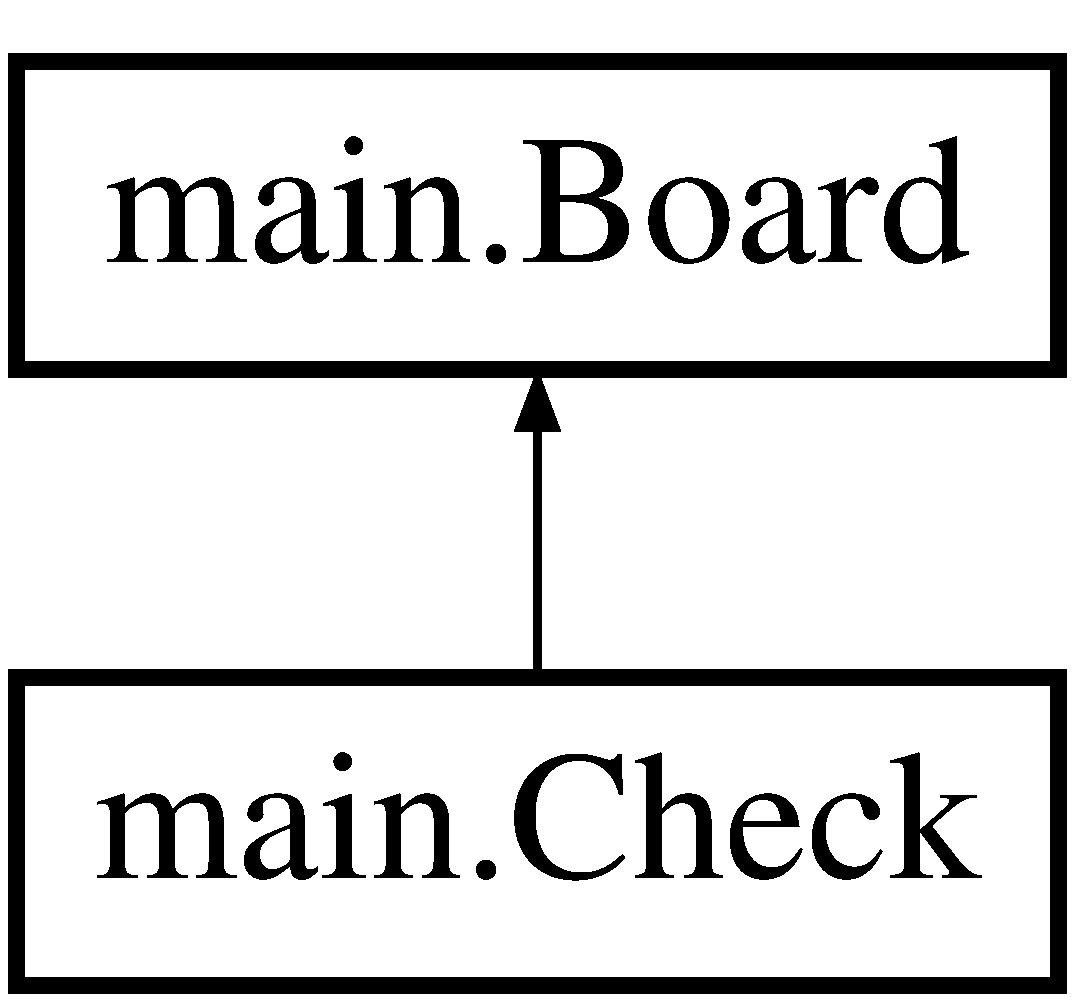
\includegraphics[height=2.000000cm]{classmain_1_1_check}
\end{center}
\end{figure}
\subsection*{Public Member Functions}
\begin{DoxyCompactItemize}
\item 
\hyperlink{classmain_1_1_check_ad50f8884f3ccd0b8dfd3b5f55f3ba08b}{Check} (boolean custom)
\item 
\hyperlink{classmain_1_1_piece}{Piece} \hyperlink{classmain_1_1_check_a4c11e37a69b51afe8318b6cd99bfbe19}{get\+King} (int player)
\item 
boolean \hyperlink{classmain_1_1_check_af22afdde9a99d951237d65b8a9d32535}{king\+Checked\+Diagonally} (\hyperlink{classmain_1_1_piece}{Piece} piece)
\item 
boolean \hyperlink{classmain_1_1_check_a5230cdb389e62d0afbff4b05af28aff0}{king\+Checked\+Linearly} (\hyperlink{classmain_1_1_piece}{Piece} piece)
\item 
\mbox{\Hypertarget{classmain_1_1_check_a38b5ebac39f0fcf08f1ade84fad2655c}\label{classmain_1_1_check_a38b5ebac39f0fcf08f1ade84fad2655c}} 
boolean {\bfseries knight\+Position\+Check} (int x, int y, int player)
\item 
boolean \hyperlink{classmain_1_1_check_ad437a473d382218735067a8ba65dddc4}{king\+Checked\+By\+Knight} (\hyperlink{classmain_1_1_piece}{Piece} piece, int player)
\item 
boolean \hyperlink{classmain_1_1_check_abb80139bcdc002c32dd5e721c490d800}{is\+Checked} (int player)
\item 
boolean \hyperlink{classmain_1_1_check_a6a22c24f1a038324813439e17bc92390}{checkmate} ()
\item 
boolean \hyperlink{classmain_1_1_check_ac4c3ae82761a5bf3649785f8e97f29ce}{stalemate} ()
\end{DoxyCompactItemize}


\subsection{Constructor \& Destructor Documentation}
\mbox{\Hypertarget{classmain_1_1_check_ad50f8884f3ccd0b8dfd3b5f55f3ba08b}\label{classmain_1_1_check_ad50f8884f3ccd0b8dfd3b5f55f3ba08b}} 
\index{main\+::\+Check@{main\+::\+Check}!Check@{Check}}
\index{Check@{Check}!main\+::\+Check@{main\+::\+Check}}
\subsubsection{\texorpdfstring{Check()}{Check()}}
{\footnotesize\ttfamily main.\+Check.\+Check (\begin{DoxyParamCaption}\item[{boolean}]{custom }\end{DoxyParamCaption})}

Constructor for the \hyperlink{classmain_1_1_check}{Check} class 

\subsection{Member Function Documentation}
\mbox{\Hypertarget{classmain_1_1_check_a6a22c24f1a038324813439e17bc92390}\label{classmain_1_1_check_a6a22c24f1a038324813439e17bc92390}} 
\index{main\+::\+Check@{main\+::\+Check}!checkmate@{checkmate}}
\index{checkmate@{checkmate}!main\+::\+Check@{main\+::\+Check}}
\subsubsection{\texorpdfstring{checkmate()}{checkmate()}}
{\footnotesize\ttfamily boolean main.\+Check.\+checkmate (\begin{DoxyParamCaption}{ }\end{DoxyParamCaption})}

Function that checks if there is a checkmate within the game \begin{DoxyReturn}{Returns}
end of the game, other player wins 
\end{DoxyReturn}
\mbox{\Hypertarget{classmain_1_1_check_a4c11e37a69b51afe8318b6cd99bfbe19}\label{classmain_1_1_check_a4c11e37a69b51afe8318b6cd99bfbe19}} 
\index{main\+::\+Check@{main\+::\+Check}!get\+King@{get\+King}}
\index{get\+King@{get\+King}!main\+::\+Check@{main\+::\+Check}}
\subsubsection{\texorpdfstring{get\+King()}{getKing()}}
{\footnotesize\ttfamily \hyperlink{classmain_1_1_piece}{Piece} main.\+Check.\+get\+King (\begin{DoxyParamCaption}\item[{int}]{player }\end{DoxyParamCaption})}

Function that returns the player\textquotesingle{}s \hyperlink{classmain_1_1_king}{King} piece, and removes the piece from the board 
\begin{DoxyParams}{Parameters}
{\em player} & the player/owner of the \hyperlink{classmain_1_1_king}{King} piece \\
\hline
\end{DoxyParams}
\begin{DoxyReturn}{Returns}
the \hyperlink{classmain_1_1_king}{King} piece, determines the end of the game 
\end{DoxyReturn}
\mbox{\Hypertarget{classmain_1_1_check_abb80139bcdc002c32dd5e721c490d800}\label{classmain_1_1_check_abb80139bcdc002c32dd5e721c490d800}} 
\index{main\+::\+Check@{main\+::\+Check}!is\+Checked@{is\+Checked}}
\index{is\+Checked@{is\+Checked}!main\+::\+Check@{main\+::\+Check}}
\subsubsection{\texorpdfstring{is\+Checked()}{isChecked()}}
{\footnotesize\ttfamily boolean main.\+Check.\+is\+Checked (\begin{DoxyParamCaption}\item[{int}]{player }\end{DoxyParamCaption})}

Function that checks whether the \hyperlink{classmain_1_1_king}{King} is checked 
\begin{DoxyParams}{Parameters}
{\em player} & the player/owner of the \hyperlink{classmain_1_1_king}{King} piece \\
\hline
\end{DoxyParams}
\begin{DoxyReturn}{Returns}

\end{DoxyReturn}
\mbox{\Hypertarget{classmain_1_1_check_ad437a473d382218735067a8ba65dddc4}\label{classmain_1_1_check_ad437a473d382218735067a8ba65dddc4}} 
\index{main\+::\+Check@{main\+::\+Check}!king\+Checked\+By\+Knight@{king\+Checked\+By\+Knight}}
\index{king\+Checked\+By\+Knight@{king\+Checked\+By\+Knight}!main\+::\+Check@{main\+::\+Check}}
\subsubsection{\texorpdfstring{king\+Checked\+By\+Knight()}{kingCheckedByKnight()}}
{\footnotesize\ttfamily boolean main.\+Check.\+king\+Checked\+By\+Knight (\begin{DoxyParamCaption}\item[{\hyperlink{classmain_1_1_piece}{Piece}}]{piece,  }\item[{int}]{player }\end{DoxyParamCaption})}

Function that checks whether the \hyperlink{classmain_1_1_king}{King} piece is in check by a \hyperlink{classmain_1_1_knight}{Knight} piece 
\begin{DoxyParams}{Parameters}
{\em piece} & the \hyperlink{classmain_1_1_knight}{Knight} piece of the other player \\
\hline
{\em player} & the other player that isn\textquotesingle{}t the owner of the \hyperlink{classmain_1_1_king}{King} piece \\
\hline
\end{DoxyParams}
\begin{DoxyReturn}{Returns}
true/false boolean whether the \hyperlink{classmain_1_1_king}{King} is in check 
\end{DoxyReturn}
\mbox{\Hypertarget{classmain_1_1_check_af22afdde9a99d951237d65b8a9d32535}\label{classmain_1_1_check_af22afdde9a99d951237d65b8a9d32535}} 
\index{main\+::\+Check@{main\+::\+Check}!king\+Checked\+Diagonally@{king\+Checked\+Diagonally}}
\index{king\+Checked\+Diagonally@{king\+Checked\+Diagonally}!main\+::\+Check@{main\+::\+Check}}
\subsubsection{\texorpdfstring{king\+Checked\+Diagonally()}{kingCheckedDiagonally()}}
{\footnotesize\ttfamily boolean main.\+Check.\+king\+Checked\+Diagonally (\begin{DoxyParamCaption}\item[{\hyperlink{classmain_1_1_piece}{Piece}}]{piece }\end{DoxyParamCaption})}

Function that checks whether the \hyperlink{classmain_1_1_king}{King} piece is in check diagonally 
\begin{DoxyParams}{Parameters}
{\em piece} & the \hyperlink{classmain_1_1_king}{King} piece \\
\hline
\end{DoxyParams}
\begin{DoxyReturn}{Returns}
true/false boolean whether the \hyperlink{classmain_1_1_king}{King} is in check 
\end{DoxyReturn}
\mbox{\Hypertarget{classmain_1_1_check_a5230cdb389e62d0afbff4b05af28aff0}\label{classmain_1_1_check_a5230cdb389e62d0afbff4b05af28aff0}} 
\index{main\+::\+Check@{main\+::\+Check}!king\+Checked\+Linearly@{king\+Checked\+Linearly}}
\index{king\+Checked\+Linearly@{king\+Checked\+Linearly}!main\+::\+Check@{main\+::\+Check}}
\subsubsection{\texorpdfstring{king\+Checked\+Linearly()}{kingCheckedLinearly()}}
{\footnotesize\ttfamily boolean main.\+Check.\+king\+Checked\+Linearly (\begin{DoxyParamCaption}\item[{\hyperlink{classmain_1_1_piece}{Piece}}]{piece }\end{DoxyParamCaption})}

Function that checks whether the \hyperlink{classmain_1_1_king}{King} piece is in check linearly 
\begin{DoxyParams}{Parameters}
{\em piece} & the \hyperlink{classmain_1_1_king}{King} piece \\
\hline
\end{DoxyParams}
\begin{DoxyReturn}{Returns}
true/false boolean whether the \hyperlink{classmain_1_1_king}{King} is in check 
\end{DoxyReturn}
\mbox{\Hypertarget{classmain_1_1_check_ac4c3ae82761a5bf3649785f8e97f29ce}\label{classmain_1_1_check_ac4c3ae82761a5bf3649785f8e97f29ce}} 
\index{main\+::\+Check@{main\+::\+Check}!stalemate@{stalemate}}
\index{stalemate@{stalemate}!main\+::\+Check@{main\+::\+Check}}
\subsubsection{\texorpdfstring{stalemate()}{stalemate()}}
{\footnotesize\ttfamily boolean main.\+Check.\+stalemate (\begin{DoxyParamCaption}{ }\end{DoxyParamCaption})}

Function that checks if there is a stalemate within the game \begin{DoxyReturn}{Returns}
end of the game, draw 
\end{DoxyReturn}


The documentation for this class was generated from the following file\+:\begin{DoxyCompactItemize}
\item 
src/main/Check.\+java\end{DoxyCompactItemize}

\hypertarget{classtest_1_1_check_test}{}\section{test.\+Check\+Test Class Reference}
\label{classtest_1_1_check_test}\index{test.\+Check\+Test@{test.\+Check\+Test}}
\subsection*{Public Member Functions}
\begin{DoxyCompactItemize}
\item 
\mbox{\Hypertarget{classtest_1_1_check_test_a8a2eee32b1cdde4e206292c3d1a72d62}\label{classtest_1_1_check_test_a8a2eee32b1cdde4e206292c3d1a72d62}} 
void {\bfseries test\+Checkmate} ()  throws Exception 
\item 
\mbox{\Hypertarget{classtest_1_1_check_test_aebcd23dbb0fe6ebcfcc97286149966b2}\label{classtest_1_1_check_test_aebcd23dbb0fe6ebcfcc97286149966b2}} 
void {\bfseries test\+Stalemate} ()  throws Exception 
\end{DoxyCompactItemize}


The documentation for this class was generated from the following file\+:\begin{DoxyCompactItemize}
\item 
src/test/Check\+Test.\+java\end{DoxyCompactItemize}

\hypertarget{class_g_u_i_1_1_game}{}\section{G\+U\+I.\+Game Class Reference}
\label{class_g_u_i_1_1_game}\index{G\+U\+I.\+Game@{G\+U\+I.\+Game}}
\subsection*{Public Member Functions}
\begin{DoxyCompactItemize}
\item 
\hyperlink{class_g_u_i_1_1_game_a97c23a5cb3fed78d68ef75d6d889b77a}{Game} ()  throws I\+O\+Exception 
\end{DoxyCompactItemize}


\subsection{Constructor \& Destructor Documentation}
\mbox{\Hypertarget{class_g_u_i_1_1_game_a97c23a5cb3fed78d68ef75d6d889b77a}\label{class_g_u_i_1_1_game_a97c23a5cb3fed78d68ef75d6d889b77a}} 
\index{G\+U\+I\+::\+Game@{G\+U\+I\+::\+Game}!Game@{Game}}
\index{Game@{Game}!G\+U\+I\+::\+Game@{G\+U\+I\+::\+Game}}
\subsubsection{\texorpdfstring{Game()}{Game()}}
{\footnotesize\ttfamily G\+U\+I.\+Game.\+Game (\begin{DoxyParamCaption}{ }\end{DoxyParamCaption}) throws I\+O\+Exception}

Constructor for the \hyperlink{class_g_u_i_1_1_game}{Game} class, which initializes the G\+UI and game board 
\begin{DoxyExceptions}{Exceptions}
{\em I\+O\+Exception} & \\
\hline
\end{DoxyExceptions}


The documentation for this class was generated from the following file\+:\begin{DoxyCompactItemize}
\item 
src/\+G\+U\+I/Game.\+java\end{DoxyCompactItemize}

\hypertarget{classmain_1_1_king}{}\section{main.\+King Class Reference}
\label{classmain_1_1_king}\index{main.\+King@{main.\+King}}
Inheritance diagram for main.\+King\+:\begin{figure}[H]
\begin{center}
\leavevmode
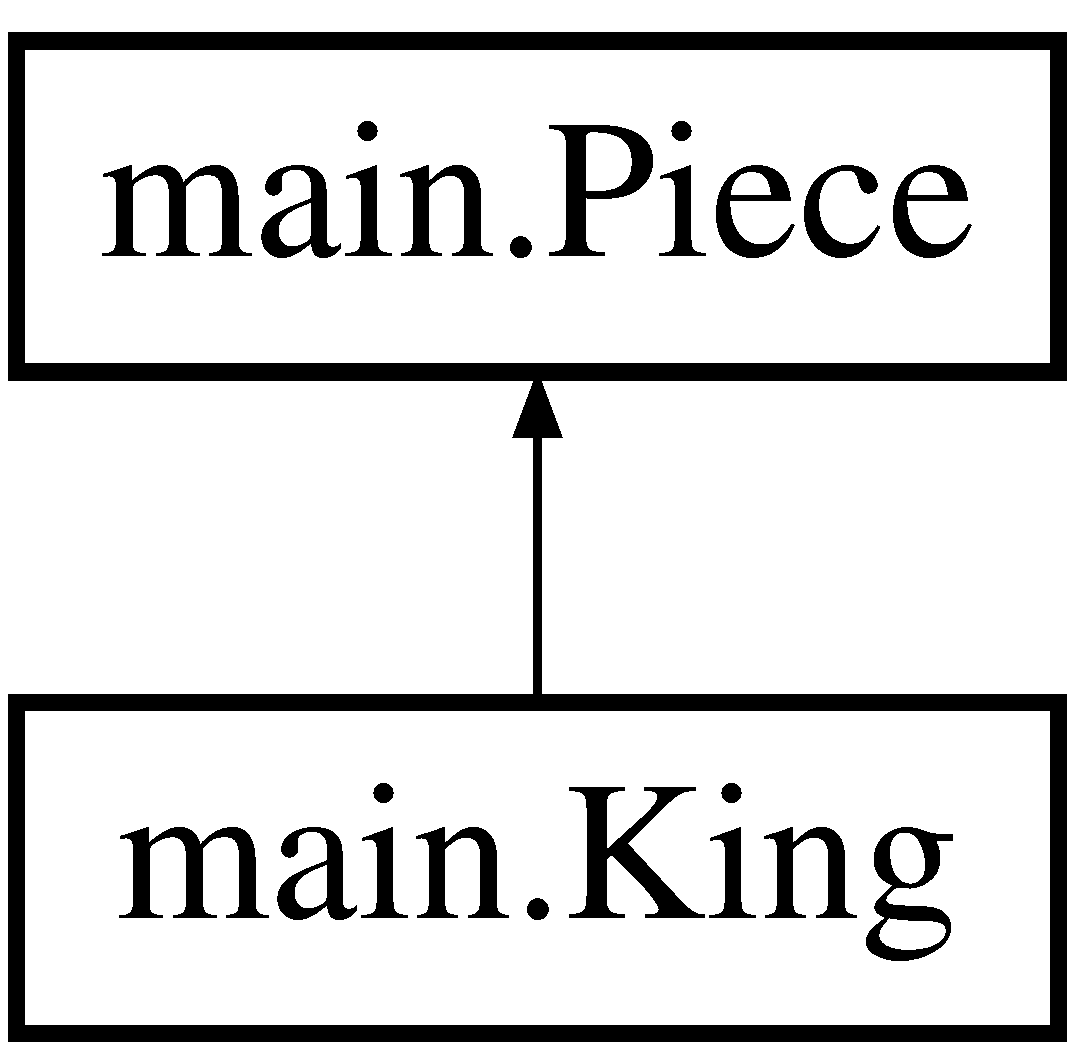
\includegraphics[height=2.000000cm]{classmain_1_1_king}
\end{center}
\end{figure}
\subsection*{Public Member Functions}
\begin{DoxyCompactItemize}
\item 
\hyperlink{classmain_1_1_king_a7512b299fe9a8b4ebcad47208403ee59}{King} (int player, \hyperlink{classmain_1_1_position}{Position} position, \hyperlink{classmain_1_1_board}{Board} board)
\item 
boolean \hyperlink{classmain_1_1_king_a96e05b09b8fb578a359fc25fc0af9b1b}{can\+Move\+To} (int x, int y)
\end{DoxyCompactItemize}


\subsection{Constructor \& Destructor Documentation}
\mbox{\Hypertarget{classmain_1_1_king_a7512b299fe9a8b4ebcad47208403ee59}\label{classmain_1_1_king_a7512b299fe9a8b4ebcad47208403ee59}} 
\index{main\+::\+King@{main\+::\+King}!King@{King}}
\index{King@{King}!main\+::\+King@{main\+::\+King}}
\subsubsection{\texorpdfstring{King()}{King()}}
{\footnotesize\ttfamily main.\+King.\+King (\begin{DoxyParamCaption}\item[{int}]{player,  }\item[{\hyperlink{classmain_1_1_position}{Position}}]{position,  }\item[{\hyperlink{classmain_1_1_board}{Board}}]{board }\end{DoxyParamCaption})}

Constructor for the \hyperlink{classmain_1_1_king}{King} class 
\begin{DoxyParams}{Parameters}
{\em player} & piece player/owner \\
\hline
{\em position} & location of the piece on the board \\
\hline
{\em board} & game board \\
\hline
\end{DoxyParams}


\subsection{Member Function Documentation}
\mbox{\Hypertarget{classmain_1_1_king_a96e05b09b8fb578a359fc25fc0af9b1b}\label{classmain_1_1_king_a96e05b09b8fb578a359fc25fc0af9b1b}} 
\index{main\+::\+King@{main\+::\+King}!can\+Move\+To@{can\+Move\+To}}
\index{can\+Move\+To@{can\+Move\+To}!main\+::\+King@{main\+::\+King}}
\subsubsection{\texorpdfstring{can\+Move\+To()}{canMoveTo()}}
{\footnotesize\ttfamily boolean main.\+King.\+can\+Move\+To (\begin{DoxyParamCaption}\item[{int}]{x,  }\item[{int}]{y }\end{DoxyParamCaption})}

Function for checking if the piece can move to a specified (x,y) position on the board 
\begin{DoxyParams}{Parameters}
{\em x} & position along the x axis \\
\hline
{\em y} & position along the y axis \\
\hline
\end{DoxyParams}
\begin{DoxyReturn}{Returns}
true/false boolean whether it\textquotesingle{}s a valid move 
\end{DoxyReturn}


The documentation for this class was generated from the following file\+:\begin{DoxyCompactItemize}
\item 
src/main/King.\+java\end{DoxyCompactItemize}

\hypertarget{classtest_1_1_king_test}{}\section{test.\+King\+Test Class Reference}
\label{classtest_1_1_king_test}\index{test.\+King\+Test@{test.\+King\+Test}}
\subsection*{Public Member Functions}
\begin{DoxyCompactItemize}
\item 
\mbox{\Hypertarget{classtest_1_1_king_test_a74ddf32132becaa57b5e0a13fa0a8623}\label{classtest_1_1_king_test_a74ddf32132becaa57b5e0a13fa0a8623}} 
void {\bfseries test\+Position} ()  throws Exception 
\item 
\mbox{\Hypertarget{classtest_1_1_king_test_af74b3f848c5b36b3fbf5ce3c2de52759}\label{classtest_1_1_king_test_af74b3f848c5b36b3fbf5ce3c2de52759}} 
void {\bfseries test\+Valid\+Move} ()  throws Exception 
\item 
\mbox{\Hypertarget{classtest_1_1_king_test_a201a47c7e35d8fa6582c6c91c62b6f03}\label{classtest_1_1_king_test_a201a47c7e35d8fa6582c6c91c62b6f03}} 
void {\bfseries test\+Invalid\+Move} ()  throws Exception 
\end{DoxyCompactItemize}


The documentation for this class was generated from the following file\+:\begin{DoxyCompactItemize}
\item 
src/test/King\+Test.\+java\end{DoxyCompactItemize}

\hypertarget{classmain_1_1_knight}{}\section{main.\+Knight Class Reference}
\label{classmain_1_1_knight}\index{main.\+Knight@{main.\+Knight}}
Inheritance diagram for main.\+Knight\+:\begin{figure}[H]
\begin{center}
\leavevmode
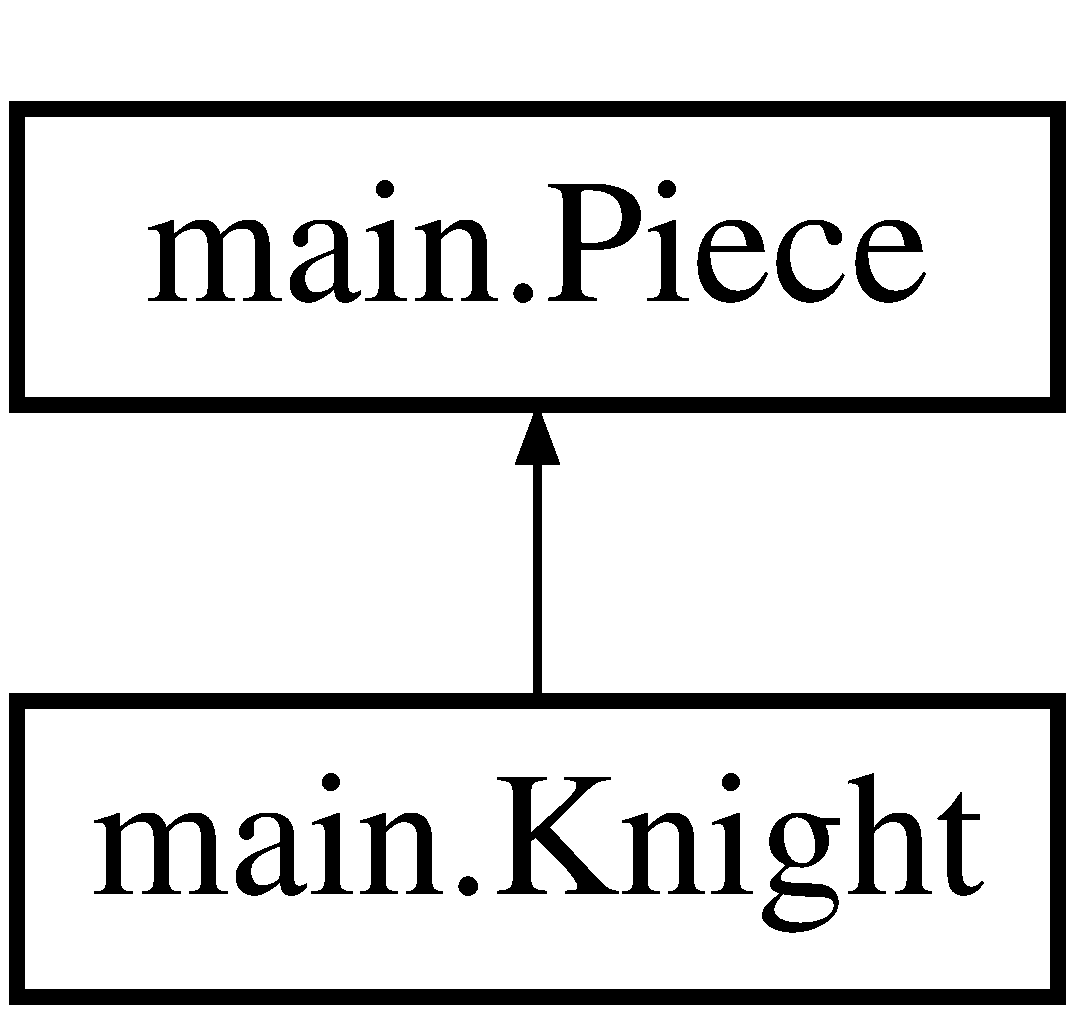
\includegraphics[height=2.000000cm]{classmain_1_1_knight}
\end{center}
\end{figure}
\subsection*{Public Member Functions}
\begin{DoxyCompactItemize}
\item 
\hyperlink{classmain_1_1_knight_a63f17a48fdb2b1d2c42a4f5c62b98aac}{Knight} (int player, \hyperlink{classmain_1_1_position}{Position} position, \hyperlink{classmain_1_1_board}{Board} board)
\item 
boolean \hyperlink{classmain_1_1_knight_a7012b51c708121845a6fc1c911a412ba}{can\+Move\+To} (int x, int y)
\end{DoxyCompactItemize}


\subsection{Constructor \& Destructor Documentation}
\mbox{\Hypertarget{classmain_1_1_knight_a63f17a48fdb2b1d2c42a4f5c62b98aac}\label{classmain_1_1_knight_a63f17a48fdb2b1d2c42a4f5c62b98aac}} 
\index{main\+::\+Knight@{main\+::\+Knight}!Knight@{Knight}}
\index{Knight@{Knight}!main\+::\+Knight@{main\+::\+Knight}}
\subsubsection{\texorpdfstring{Knight()}{Knight()}}
{\footnotesize\ttfamily main.\+Knight.\+Knight (\begin{DoxyParamCaption}\item[{int}]{player,  }\item[{\hyperlink{classmain_1_1_position}{Position}}]{position,  }\item[{\hyperlink{classmain_1_1_board}{Board}}]{board }\end{DoxyParamCaption})}

Constructor for the \hyperlink{classmain_1_1_knight}{Knight} class 
\begin{DoxyParams}{Parameters}
{\em player} & piece player/owner \\
\hline
{\em position} & location of the piece on the board \\
\hline
{\em board} & game board \\
\hline
\end{DoxyParams}


\subsection{Member Function Documentation}
\mbox{\Hypertarget{classmain_1_1_knight_a7012b51c708121845a6fc1c911a412ba}\label{classmain_1_1_knight_a7012b51c708121845a6fc1c911a412ba}} 
\index{main\+::\+Knight@{main\+::\+Knight}!can\+Move\+To@{can\+Move\+To}}
\index{can\+Move\+To@{can\+Move\+To}!main\+::\+Knight@{main\+::\+Knight}}
\subsubsection{\texorpdfstring{can\+Move\+To()}{canMoveTo()}}
{\footnotesize\ttfamily boolean main.\+Knight.\+can\+Move\+To (\begin{DoxyParamCaption}\item[{int}]{x,  }\item[{int}]{y }\end{DoxyParamCaption})}

Function for checking if the piece can move to a specified (x,y) position on the board 
\begin{DoxyParams}{Parameters}
{\em x} & position along the x axis \\
\hline
{\em y} & position along the y axis \\
\hline
\end{DoxyParams}
\begin{DoxyReturn}{Returns}
true/false boolean whether it\textquotesingle{}s a valid move 
\end{DoxyReturn}


The documentation for this class was generated from the following file\+:\begin{DoxyCompactItemize}
\item 
src/main/Knight.\+java\end{DoxyCompactItemize}

\hypertarget{classtest_1_1_knight_test}{}\section{test.\+Knight\+Test Class Reference}
\label{classtest_1_1_knight_test}\index{test.\+Knight\+Test@{test.\+Knight\+Test}}
\subsection*{Public Member Functions}
\begin{DoxyCompactItemize}
\item 
\mbox{\Hypertarget{classtest_1_1_knight_test_a29bd8fee71c95dd45953f31ac6a8fef5}\label{classtest_1_1_knight_test_a29bd8fee71c95dd45953f31ac6a8fef5}} 
void {\bfseries test\+Position} ()  throws Exception 
\item 
\mbox{\Hypertarget{classtest_1_1_knight_test_aeaa3eef48cceb07d146943e346e6f170}\label{classtest_1_1_knight_test_aeaa3eef48cceb07d146943e346e6f170}} 
void {\bfseries test\+Valid\+Move} ()  throws Exception 
\item 
\mbox{\Hypertarget{classtest_1_1_knight_test_a4feaa624058603101178188b8bcf223e}\label{classtest_1_1_knight_test_a4feaa624058603101178188b8bcf223e}} 
void {\bfseries test\+Invalid\+Move} ()  throws Exception 
\end{DoxyCompactItemize}


The documentation for this class was generated from the following file\+:\begin{DoxyCompactItemize}
\item 
src/test/Knight\+Test.\+java\end{DoxyCompactItemize}

\hypertarget{class_main}{}\section{Main Class Reference}
\label{class_main}\index{Main@{Main}}
\subsection*{Static Public Member Functions}
\begin{DoxyCompactItemize}
\item 
\mbox{\Hypertarget{class_main_a8df768461f886ac6b6051146e3e10c4d}\label{class_main_a8df768461f886ac6b6051146e3e10c4d}} 
static void {\bfseries main} (String \mbox{[}$\,$\mbox{]}args)  throws I\+O\+Exception 
\end{DoxyCompactItemize}


The documentation for this class was generated from the following file\+:\begin{DoxyCompactItemize}
\item 
src/Main.\+java\end{DoxyCompactItemize}

\hypertarget{classmain_1_1_pawn}{}\section{main.\+Pawn Class Reference}
\label{classmain_1_1_pawn}\index{main.\+Pawn@{main.\+Pawn}}
Inheritance diagram for main.\+Pawn\+:\begin{figure}[H]
\begin{center}
\leavevmode
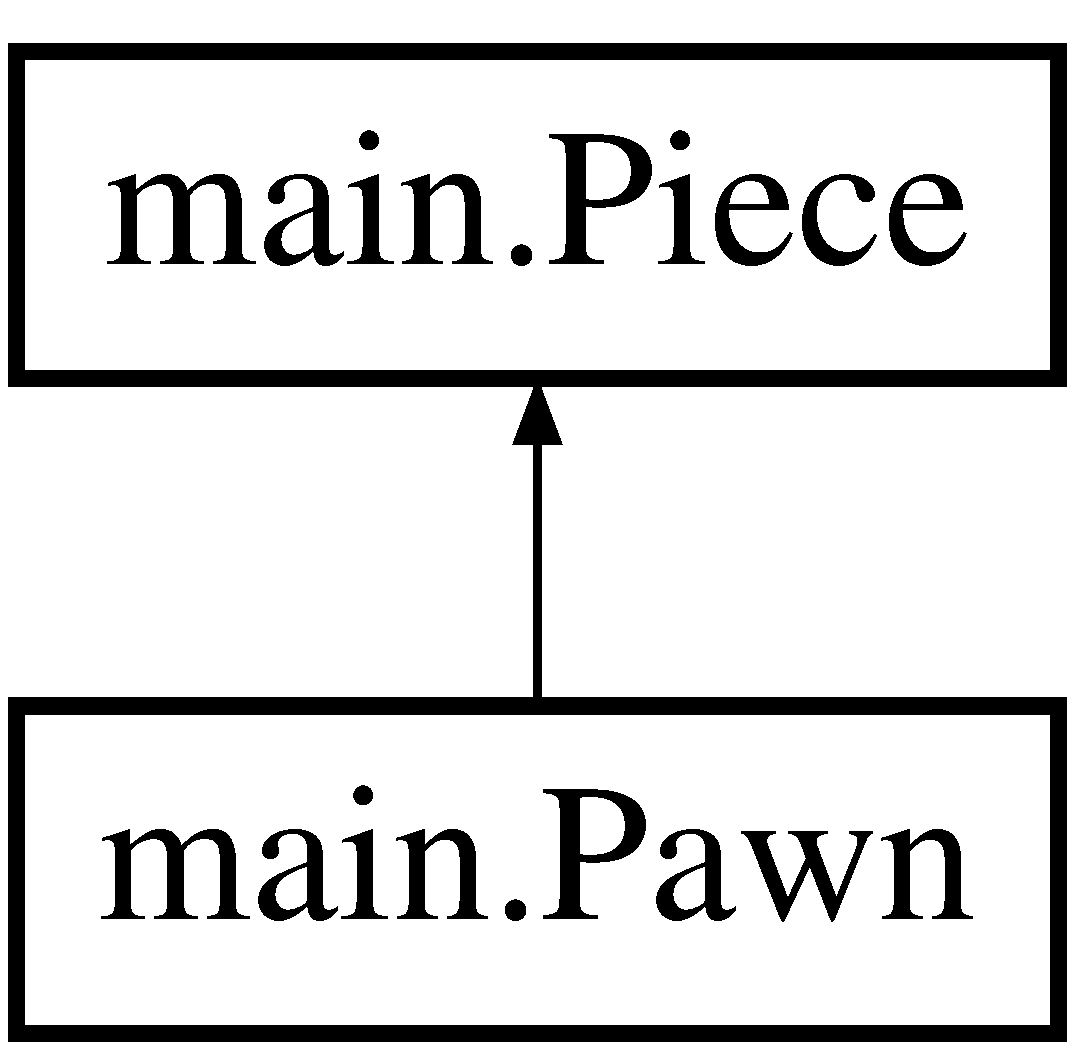
\includegraphics[height=2.000000cm]{classmain_1_1_pawn}
\end{center}
\end{figure}
\subsection*{Public Member Functions}
\begin{DoxyCompactItemize}
\item 
\hyperlink{classmain_1_1_pawn_a4852bea50e9ece41201fdd0e516611b7}{Pawn} (int player, \hyperlink{classmain_1_1_position}{Position} position, \hyperlink{classmain_1_1_board}{Board} board)
\item 
boolean \hyperlink{classmain_1_1_pawn_a22a9e6be922fa7333ac79f2ab5a327b6}{can\+Move\+To} (int x, int y)
\end{DoxyCompactItemize}


\subsection{Constructor \& Destructor Documentation}
\mbox{\Hypertarget{classmain_1_1_pawn_a4852bea50e9ece41201fdd0e516611b7}\label{classmain_1_1_pawn_a4852bea50e9ece41201fdd0e516611b7}} 
\index{main\+::\+Pawn@{main\+::\+Pawn}!Pawn@{Pawn}}
\index{Pawn@{Pawn}!main\+::\+Pawn@{main\+::\+Pawn}}
\subsubsection{\texorpdfstring{Pawn()}{Pawn()}}
{\footnotesize\ttfamily main.\+Pawn.\+Pawn (\begin{DoxyParamCaption}\item[{int}]{player,  }\item[{\hyperlink{classmain_1_1_position}{Position}}]{position,  }\item[{\hyperlink{classmain_1_1_board}{Board}}]{board }\end{DoxyParamCaption})}

Constructor for the \hyperlink{classmain_1_1_pawn}{Pawn} class 
\begin{DoxyParams}{Parameters}
{\em player} & piece player/owner \\
\hline
{\em position} & location of the piece on the board \\
\hline
{\em board} & game board \\
\hline
\end{DoxyParams}


\subsection{Member Function Documentation}
\mbox{\Hypertarget{classmain_1_1_pawn_a22a9e6be922fa7333ac79f2ab5a327b6}\label{classmain_1_1_pawn_a22a9e6be922fa7333ac79f2ab5a327b6}} 
\index{main\+::\+Pawn@{main\+::\+Pawn}!can\+Move\+To@{can\+Move\+To}}
\index{can\+Move\+To@{can\+Move\+To}!main\+::\+Pawn@{main\+::\+Pawn}}
\subsubsection{\texorpdfstring{can\+Move\+To()}{canMoveTo()}}
{\footnotesize\ttfamily boolean main.\+Pawn.\+can\+Move\+To (\begin{DoxyParamCaption}\item[{int}]{x,  }\item[{int}]{y }\end{DoxyParamCaption})}

Function for checking if the piece can move to a specified (x,y) position on the board 
\begin{DoxyParams}{Parameters}
{\em x} & position along the x axis \\
\hline
{\em y} & position along the y axis \\
\hline
\end{DoxyParams}
\begin{DoxyReturn}{Returns}
true/false boolean whether it\textquotesingle{}s a valid move 
\end{DoxyReturn}


The documentation for this class was generated from the following file\+:\begin{DoxyCompactItemize}
\item 
src/main/Pawn.\+java\end{DoxyCompactItemize}

\hypertarget{classtest_1_1_pawn_test}{}\section{test.\+Pawn\+Test Class Reference}
\label{classtest_1_1_pawn_test}\index{test.\+Pawn\+Test@{test.\+Pawn\+Test}}
\subsection*{Public Member Functions}
\begin{DoxyCompactItemize}
\item 
\mbox{\Hypertarget{classtest_1_1_pawn_test_a843453c706973021b99499f44c891e6a}\label{classtest_1_1_pawn_test_a843453c706973021b99499f44c891e6a}} 
void {\bfseries test\+Position} ()  throws Exception 
\item 
\mbox{\Hypertarget{classtest_1_1_pawn_test_ab015d6288131fcc3be0db85c96bf926e}\label{classtest_1_1_pawn_test_ab015d6288131fcc3be0db85c96bf926e}} 
void {\bfseries test\+Valid\+Move} ()  throws Exception 
\item 
\mbox{\Hypertarget{classtest_1_1_pawn_test_a8d47ac0e26d59ad405fdc834a16bd220}\label{classtest_1_1_pawn_test_a8d47ac0e26d59ad405fdc834a16bd220}} 
void {\bfseries test\+Invalid\+Move} ()  throws Exception 
\end{DoxyCompactItemize}


The documentation for this class was generated from the following file\+:\begin{DoxyCompactItemize}
\item 
src/test/Pawn\+Test.\+java\end{DoxyCompactItemize}

\hypertarget{classmain_1_1_piece}{}\section{main.\+Piece Class Reference}
\label{classmain_1_1_piece}\index{main.\+Piece@{main.\+Piece}}
Inheritance diagram for main.\+Piece\+:\begin{figure}[H]
\begin{center}
\leavevmode
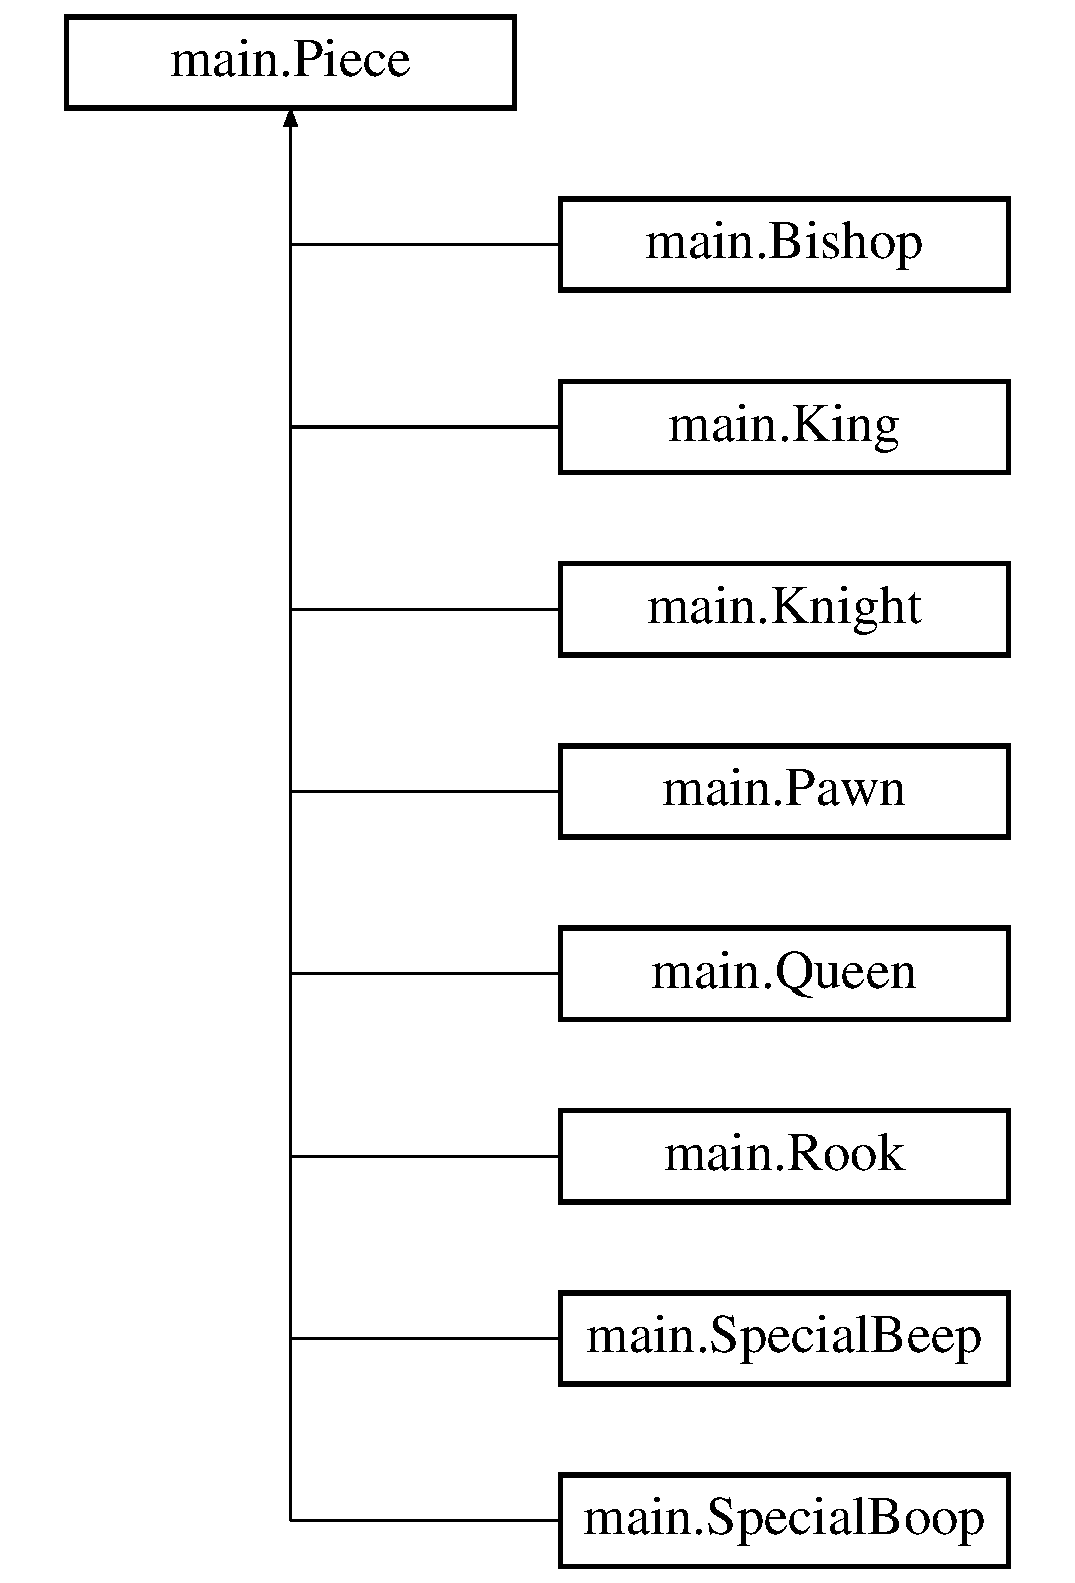
\includegraphics[height=9.000000cm]{classmain_1_1_piece}
\end{center}
\end{figure}
\subsection*{Public Member Functions}
\begin{DoxyCompactItemize}
\item 
\hyperlink{classmain_1_1_piece_a02a26b5661817cccd3f07d63349144f8}{Piece} (int player, \hyperlink{classmain_1_1_position}{Position} position, \hyperlink{classmain_1_1_board}{Board} board)
\item 
\mbox{\Hypertarget{classmain_1_1_piece_aa5b9e15c472cd58753a5b7db76666ed0}\label{classmain_1_1_piece_aa5b9e15c472cd58753a5b7db76666ed0}} 
int {\bfseries get\+Player} ()
\item 
\mbox{\Hypertarget{classmain_1_1_piece_a609b995790e8ce5ac6150d43765f33e6}\label{classmain_1_1_piece_a609b995790e8ce5ac6150d43765f33e6}} 
\hyperlink{classmain_1_1_position}{Position} {\bfseries get\+Position} ()
\item 
\mbox{\Hypertarget{classmain_1_1_piece_ac64b94e395aeccaa7775f64347008942}\label{classmain_1_1_piece_ac64b94e395aeccaa7775f64347008942}} 
int {\bfseries get\+Row} ()
\item 
\mbox{\Hypertarget{classmain_1_1_piece_a8bd82e7f1f966d64d6ae71ea6a1b2866}\label{classmain_1_1_piece_a8bd82e7f1f966d64d6ae71ea6a1b2866}} 
int {\bfseries get\+Col} ()
\item 
\mbox{\Hypertarget{classmain_1_1_piece_a4379392982c94b448a00c4a83f3d5552}\label{classmain_1_1_piece_a4379392982c94b448a00c4a83f3d5552}} 
\hyperlink{classmain_1_1_board}{Board} {\bfseries get\+Board} ()
\item 
\mbox{\Hypertarget{classmain_1_1_piece_af64fbce8fc1e520849595a2e902f0db3}\label{classmain_1_1_piece_af64fbce8fc1e520849595a2e902f0db3}} 
void {\bfseries set\+Player} (int player)
\item 
\mbox{\Hypertarget{classmain_1_1_piece_a1b2f7b9dc5c716c353937849d26d2def}\label{classmain_1_1_piece_a1b2f7b9dc5c716c353937849d26d2def}} 
void {\bfseries set\+Board} (\hyperlink{classmain_1_1_board}{Board} board)
\item 
\mbox{\Hypertarget{classmain_1_1_piece_a25386672406846164d702a0dedb29eaf}\label{classmain_1_1_piece_a25386672406846164d702a0dedb29eaf}} 
void {\bfseries set\+Position} (\hyperlink{classmain_1_1_position}{Position} position)
\item 
\mbox{\Hypertarget{classmain_1_1_piece_ae3d8f5049a959c98cc3e1c11fe071603}\label{classmain_1_1_piece_ae3d8f5049a959c98cc3e1c11fe071603}} 
boolean {\bfseries out\+Of\+Bounds} (int x, int y)
\item 
boolean \hyperlink{classmain_1_1_piece_a9155e5be2c034abe7c87aa6c2410cdfb}{valid\+Move} (int x, int y, int xi, int yi)
\end{DoxyCompactItemize}


\subsection{Constructor \& Destructor Documentation}
\mbox{\Hypertarget{classmain_1_1_piece_a02a26b5661817cccd3f07d63349144f8}\label{classmain_1_1_piece_a02a26b5661817cccd3f07d63349144f8}} 
\index{main\+::\+Piece@{main\+::\+Piece}!Piece@{Piece}}
\index{Piece@{Piece}!main\+::\+Piece@{main\+::\+Piece}}
\subsubsection{\texorpdfstring{Piece()}{Piece()}}
{\footnotesize\ttfamily main.\+Piece.\+Piece (\begin{DoxyParamCaption}\item[{int}]{player,  }\item[{\hyperlink{classmain_1_1_position}{Position}}]{position,  }\item[{\hyperlink{classmain_1_1_board}{Board}}]{board }\end{DoxyParamCaption})}

Constructor for the \hyperlink{classmain_1_1_piece}{Piece} class 
\begin{DoxyParams}{Parameters}
{\em player} & \\
\hline
{\em position} & \\
\hline
{\em board} & \\
\hline
\end{DoxyParams}


\subsection{Member Function Documentation}
\mbox{\Hypertarget{classmain_1_1_piece_a9155e5be2c034abe7c87aa6c2410cdfb}\label{classmain_1_1_piece_a9155e5be2c034abe7c87aa6c2410cdfb}} 
\index{main\+::\+Piece@{main\+::\+Piece}!valid\+Move@{valid\+Move}}
\index{valid\+Move@{valid\+Move}!main\+::\+Piece@{main\+::\+Piece}}
\subsubsection{\texorpdfstring{valid\+Move()}{validMove()}}
{\footnotesize\ttfamily boolean main.\+Piece.\+valid\+Move (\begin{DoxyParamCaption}\item[{int}]{x,  }\item[{int}]{y,  }\item[{int}]{xi,  }\item[{int}]{yi }\end{DoxyParamCaption})}

Function that checks whether a specified position on the board is a valid position to move to 
\begin{DoxyParams}{Parameters}
{\em x} & position along the x axis of the desired position \\
\hline
{\em y} & position along the y axis of the desired position \\
\hline
{\em xi} & position along the x axis of the initial position \\
\hline
{\em yi} & position along the y axis of the initial position \\
\hline
\end{DoxyParams}
\begin{DoxyReturn}{Returns}
true/false boolean whether the move is valid 
\end{DoxyReturn}


The documentation for this class was generated from the following file\+:\begin{DoxyCompactItemize}
\item 
src/main/Piece.\+java\end{DoxyCompactItemize}

\hypertarget{classmain_1_1_position}{}\section{main.\+Position Class Reference}
\label{classmain_1_1_position}\index{main.\+Position@{main.\+Position}}
\subsection*{Public Member Functions}
\begin{DoxyCompactItemize}
\item 
\mbox{\Hypertarget{classmain_1_1_position_ab8490181c1618fd65161fa5efcaa4ee9}\label{classmain_1_1_position_ab8490181c1618fd65161fa5efcaa4ee9}} 
{\bfseries Position} (int x, int y)
\item 
\mbox{\Hypertarget{classmain_1_1_position_a87cabaf4efc7d90cb344b624978fa18e}\label{classmain_1_1_position_a87cabaf4efc7d90cb344b624978fa18e}} 
int {\bfseries get\+Row} ()
\item 
\mbox{\Hypertarget{classmain_1_1_position_abb732f753b21fc6bc2bcf18eb49e0e0d}\label{classmain_1_1_position_abb732f753b21fc6bc2bcf18eb49e0e0d}} 
int {\bfseries get\+Col} ()
\end{DoxyCompactItemize}


The documentation for this class was generated from the following file\+:\begin{DoxyCompactItemize}
\item 
src/main/Position.\+java\end{DoxyCompactItemize}

\hypertarget{classmain_1_1_queen}{}\section{main.\+Queen Class Reference}
\label{classmain_1_1_queen}\index{main.\+Queen@{main.\+Queen}}
Inheritance diagram for main.\+Queen\+:\begin{figure}[H]
\begin{center}
\leavevmode
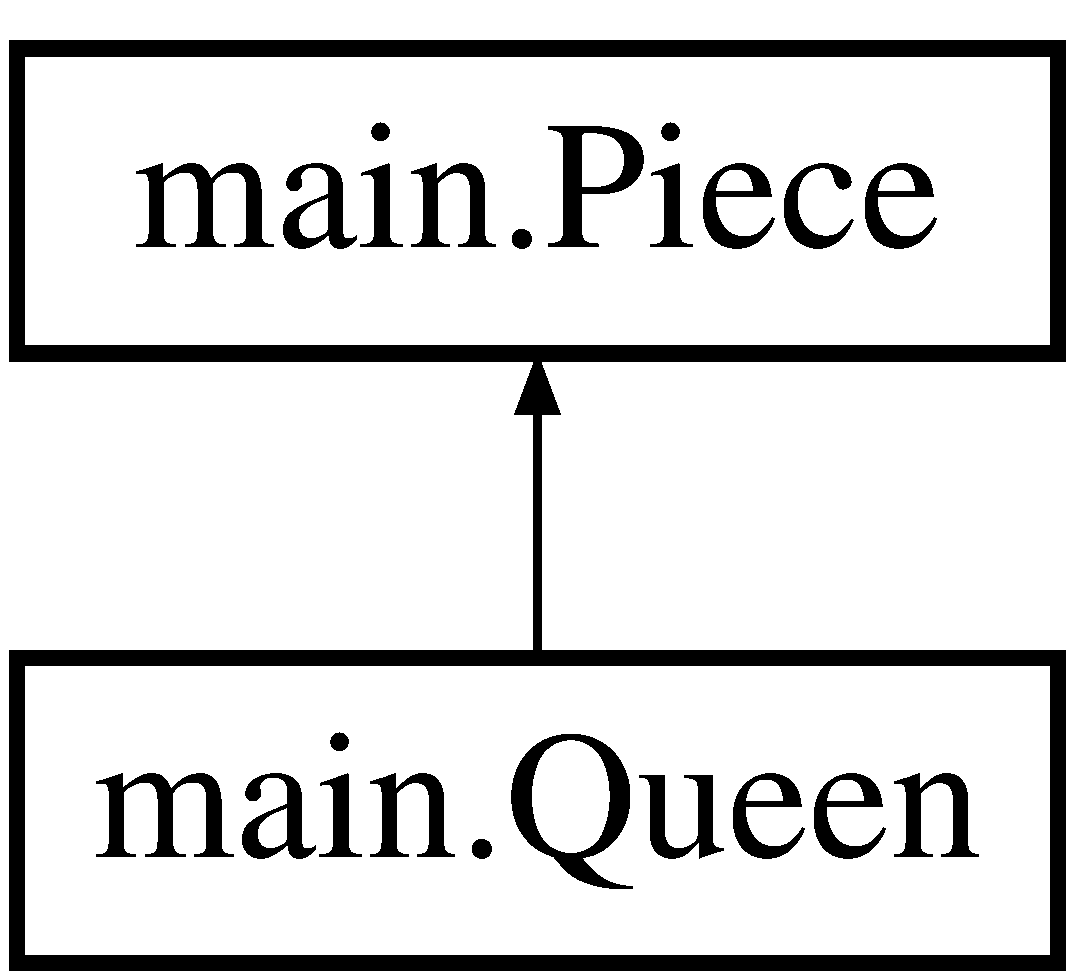
\includegraphics[height=2.000000cm]{classmain_1_1_queen}
\end{center}
\end{figure}
\subsection*{Public Member Functions}
\begin{DoxyCompactItemize}
\item 
\hyperlink{classmain_1_1_queen_a421f06bd817355da26730ba2c9b87dc1}{Queen} (int player, \hyperlink{classmain_1_1_position}{Position} position, \hyperlink{classmain_1_1_board}{Board} board)
\item 
boolean \hyperlink{classmain_1_1_queen_a9cfd9c6f093ffad8c10d9fba088595dc}{can\+Move\+To} (int x, int y)
\end{DoxyCompactItemize}


\subsection{Constructor \& Destructor Documentation}
\mbox{\Hypertarget{classmain_1_1_queen_a421f06bd817355da26730ba2c9b87dc1}\label{classmain_1_1_queen_a421f06bd817355da26730ba2c9b87dc1}} 
\index{main\+::\+Queen@{main\+::\+Queen}!Queen@{Queen}}
\index{Queen@{Queen}!main\+::\+Queen@{main\+::\+Queen}}
\subsubsection{\texorpdfstring{Queen()}{Queen()}}
{\footnotesize\ttfamily main.\+Queen.\+Queen (\begin{DoxyParamCaption}\item[{int}]{player,  }\item[{\hyperlink{classmain_1_1_position}{Position}}]{position,  }\item[{\hyperlink{classmain_1_1_board}{Board}}]{board }\end{DoxyParamCaption})}

Constructor for the \hyperlink{classmain_1_1_queen}{Queen} class 
\begin{DoxyParams}{Parameters}
{\em player} & piece player/owner \\
\hline
{\em position} & location of the piece on the board \\
\hline
{\em board} & game board \\
\hline
\end{DoxyParams}


\subsection{Member Function Documentation}
\mbox{\Hypertarget{classmain_1_1_queen_a9cfd9c6f093ffad8c10d9fba088595dc}\label{classmain_1_1_queen_a9cfd9c6f093ffad8c10d9fba088595dc}} 
\index{main\+::\+Queen@{main\+::\+Queen}!can\+Move\+To@{can\+Move\+To}}
\index{can\+Move\+To@{can\+Move\+To}!main\+::\+Queen@{main\+::\+Queen}}
\subsubsection{\texorpdfstring{can\+Move\+To()}{canMoveTo()}}
{\footnotesize\ttfamily boolean main.\+Queen.\+can\+Move\+To (\begin{DoxyParamCaption}\item[{int}]{x,  }\item[{int}]{y }\end{DoxyParamCaption})}

Function for checking if the piece can move to a specified (x,y) position on the board 
\begin{DoxyParams}{Parameters}
{\em x} & position along the x axis \\
\hline
{\em y} & position along the y axis \\
\hline
\end{DoxyParams}
\begin{DoxyReturn}{Returns}
true/false boolean whether it\textquotesingle{}s a valid move 
\end{DoxyReturn}


The documentation for this class was generated from the following file\+:\begin{DoxyCompactItemize}
\item 
src/main/Queen.\+java\end{DoxyCompactItemize}

\hypertarget{classtest_1_1_queen_test}{}\section{test.\+Queen\+Test Class Reference}
\label{classtest_1_1_queen_test}\index{test.\+Queen\+Test@{test.\+Queen\+Test}}
\subsection*{Public Member Functions}
\begin{DoxyCompactItemize}
\item 
\mbox{\Hypertarget{classtest_1_1_queen_test_aabbf0e42036c2ff1b09f22c3a5b7ffe8}\label{classtest_1_1_queen_test_aabbf0e42036c2ff1b09f22c3a5b7ffe8}} 
void {\bfseries test\+Position} ()  throws Exception 
\item 
\mbox{\Hypertarget{classtest_1_1_queen_test_aa078634711194ba68c6fb369a3977a26}\label{classtest_1_1_queen_test_aa078634711194ba68c6fb369a3977a26}} 
void {\bfseries test\+Valid\+Move} ()  throws Exception 
\item 
\mbox{\Hypertarget{classtest_1_1_queen_test_ab2bf06f0a33bf23eac9b28834ac0563c}\label{classtest_1_1_queen_test_ab2bf06f0a33bf23eac9b28834ac0563c}} 
void {\bfseries test\+Invalid\+Move} ()  throws Exception 
\end{DoxyCompactItemize}


The documentation for this class was generated from the following file\+:\begin{DoxyCompactItemize}
\item 
src/test/Queen\+Test.\+java\end{DoxyCompactItemize}

\hypertarget{classmain_1_1_rook}{}\section{main.\+Rook Class Reference}
\label{classmain_1_1_rook}\index{main.\+Rook@{main.\+Rook}}
Inheritance diagram for main.\+Rook\+:\begin{figure}[H]
\begin{center}
\leavevmode
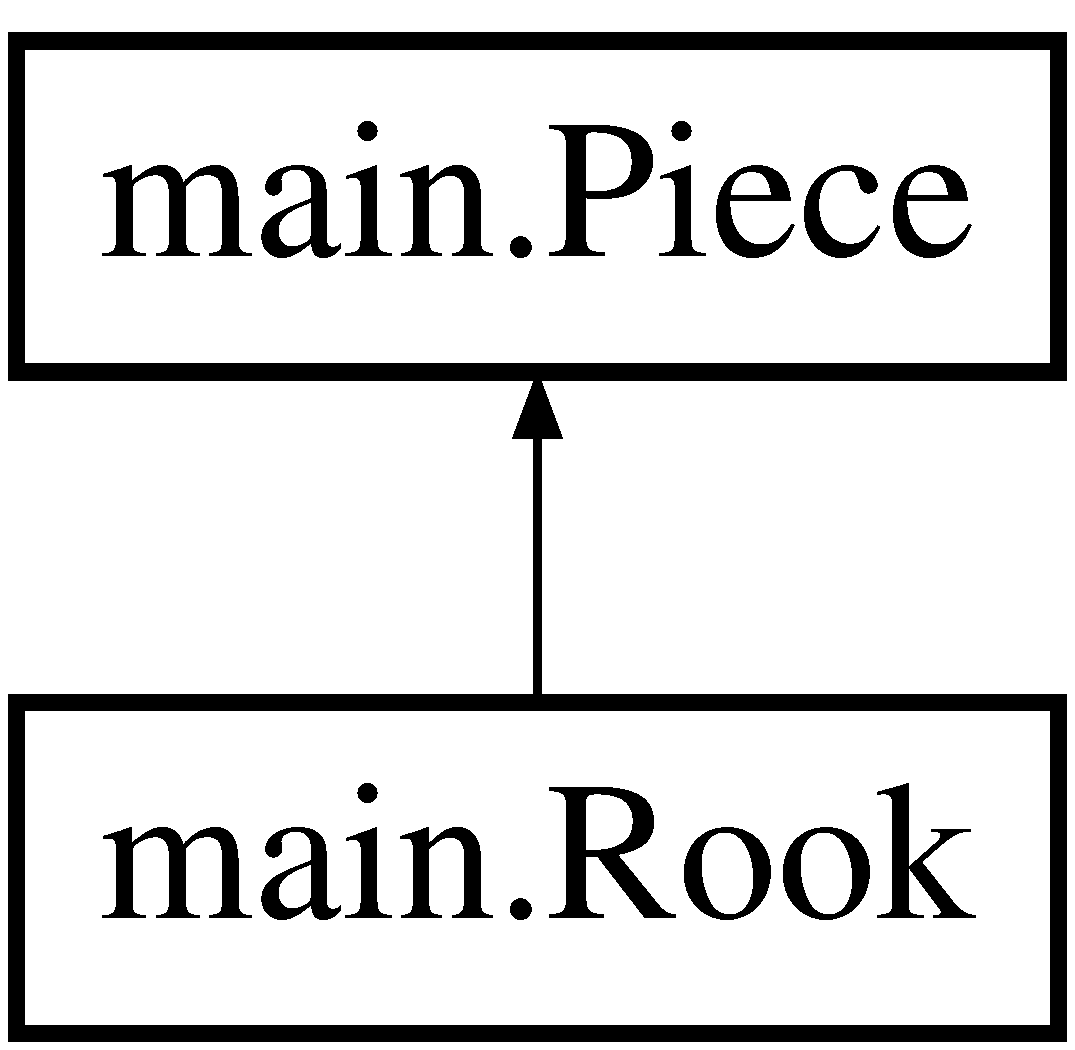
\includegraphics[height=2.000000cm]{classmain_1_1_rook}
\end{center}
\end{figure}
\subsection*{Public Member Functions}
\begin{DoxyCompactItemize}
\item 
\hyperlink{classmain_1_1_rook_a529075916777b2174122f592d3366d90}{Rook} (int player, \hyperlink{classmain_1_1_position}{Position} position, \hyperlink{classmain_1_1_board}{Board} board)
\item 
boolean \hyperlink{classmain_1_1_rook_a91848ddd38f797d23ab1be23d357fef7}{can\+Move\+To} (int x, int y)
\end{DoxyCompactItemize}


\subsection{Constructor \& Destructor Documentation}
\mbox{\Hypertarget{classmain_1_1_rook_a529075916777b2174122f592d3366d90}\label{classmain_1_1_rook_a529075916777b2174122f592d3366d90}} 
\index{main\+::\+Rook@{main\+::\+Rook}!Rook@{Rook}}
\index{Rook@{Rook}!main\+::\+Rook@{main\+::\+Rook}}
\subsubsection{\texorpdfstring{Rook()}{Rook()}}
{\footnotesize\ttfamily main.\+Rook.\+Rook (\begin{DoxyParamCaption}\item[{int}]{player,  }\item[{\hyperlink{classmain_1_1_position}{Position}}]{position,  }\item[{\hyperlink{classmain_1_1_board}{Board}}]{board }\end{DoxyParamCaption})}

Constructor for the \hyperlink{classmain_1_1_rook}{Rook} class 
\begin{DoxyParams}{Parameters}
{\em player} & piece player/owner \\
\hline
{\em position} & location of the piece on the board \\
\hline
{\em board} & game board \\
\hline
\end{DoxyParams}


\subsection{Member Function Documentation}
\mbox{\Hypertarget{classmain_1_1_rook_a91848ddd38f797d23ab1be23d357fef7}\label{classmain_1_1_rook_a91848ddd38f797d23ab1be23d357fef7}} 
\index{main\+::\+Rook@{main\+::\+Rook}!can\+Move\+To@{can\+Move\+To}}
\index{can\+Move\+To@{can\+Move\+To}!main\+::\+Rook@{main\+::\+Rook}}
\subsubsection{\texorpdfstring{can\+Move\+To()}{canMoveTo()}}
{\footnotesize\ttfamily boolean main.\+Rook.\+can\+Move\+To (\begin{DoxyParamCaption}\item[{int}]{x,  }\item[{int}]{y }\end{DoxyParamCaption})}

Function for checking if the piece can move to a specified (x,y) position on the board 
\begin{DoxyParams}{Parameters}
{\em x} & position along the x axis \\
\hline
{\em y} & position along the y axis \\
\hline
\end{DoxyParams}
\begin{DoxyReturn}{Returns}
true/false boolean whether it\textquotesingle{}s a valid move 
\end{DoxyReturn}


The documentation for this class was generated from the following file\+:\begin{DoxyCompactItemize}
\item 
src/main/Rook.\+java\end{DoxyCompactItemize}

\hypertarget{classtest_1_1_rook_test}{}\section{test.\+Rook\+Test Class Reference}
\label{classtest_1_1_rook_test}\index{test.\+Rook\+Test@{test.\+Rook\+Test}}
\subsection*{Public Member Functions}
\begin{DoxyCompactItemize}
\item 
\mbox{\Hypertarget{classtest_1_1_rook_test_a12762a0f3bc2a9f2ac4d7fa2178beb45}\label{classtest_1_1_rook_test_a12762a0f3bc2a9f2ac4d7fa2178beb45}} 
void {\bfseries test\+Position} ()  throws Exception 
\item 
\mbox{\Hypertarget{classtest_1_1_rook_test_a7c7fad4bba4ee9fa3bfb099824aff7ba}\label{classtest_1_1_rook_test_a7c7fad4bba4ee9fa3bfb099824aff7ba}} 
void {\bfseries test\+Valid\+Move} ()  throws Exception 
\item 
\mbox{\Hypertarget{classtest_1_1_rook_test_acf986d8d88f1638cdbfc369eaa5783b0}\label{classtest_1_1_rook_test_acf986d8d88f1638cdbfc369eaa5783b0}} 
void {\bfseries test\+Invalid\+Move} ()  throws Exception 
\end{DoxyCompactItemize}


The documentation for this class was generated from the following file\+:\begin{DoxyCompactItemize}
\item 
src/test/Rook\+Test.\+java\end{DoxyCompactItemize}

\hypertarget{classmain_1_1_special_beep}{}\section{main.\+Special\+Beep Class Reference}
\label{classmain_1_1_special_beep}\index{main.\+Special\+Beep@{main.\+Special\+Beep}}
Inheritance diagram for main.\+Special\+Beep\+:\begin{figure}[H]
\begin{center}
\leavevmode
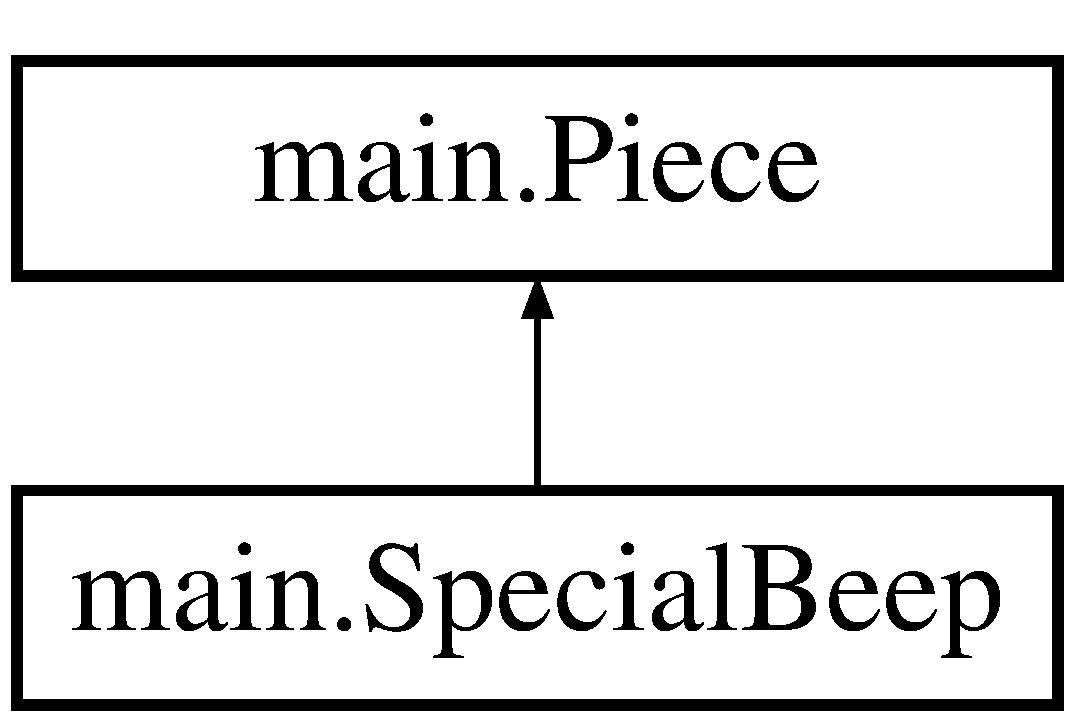
\includegraphics[height=2.000000cm]{classmain_1_1_special_beep}
\end{center}
\end{figure}
\subsection*{Public Member Functions}
\begin{DoxyCompactItemize}
\item 
\hyperlink{classmain_1_1_special_beep_a7908b98b0a1c1360e803f92940034953}{Special\+Beep} (int player, \hyperlink{classmain_1_1_position}{Position} position, \hyperlink{classmain_1_1_board}{Board} board)
\item 
boolean \hyperlink{classmain_1_1_special_beep_a2065d7405cfb1d9b49d94a55123ebd35}{can\+Move\+To} (int x, int y)
\end{DoxyCompactItemize}


\subsection{Constructor \& Destructor Documentation}
\mbox{\Hypertarget{classmain_1_1_special_beep_a7908b98b0a1c1360e803f92940034953}\label{classmain_1_1_special_beep_a7908b98b0a1c1360e803f92940034953}} 
\index{main\+::\+Special\+Beep@{main\+::\+Special\+Beep}!Special\+Beep@{Special\+Beep}}
\index{Special\+Beep@{Special\+Beep}!main\+::\+Special\+Beep@{main\+::\+Special\+Beep}}
\subsubsection{\texorpdfstring{Special\+Beep()}{SpecialBeep()}}
{\footnotesize\ttfamily main.\+Special\+Beep.\+Special\+Beep (\begin{DoxyParamCaption}\item[{int}]{player,  }\item[{\hyperlink{classmain_1_1_position}{Position}}]{position,  }\item[{\hyperlink{classmain_1_1_board}{Board}}]{board }\end{DoxyParamCaption})}

Constructor for the \hyperlink{classmain_1_1_special_beep}{Special\+Beep} class 
\begin{DoxyParams}{Parameters}
{\em player} & piece player/owner \\
\hline
{\em position} & location of the piece on the board \\
\hline
{\em board} & game board \\
\hline
\end{DoxyParams}


\subsection{Member Function Documentation}
\mbox{\Hypertarget{classmain_1_1_special_beep_a2065d7405cfb1d9b49d94a55123ebd35}\label{classmain_1_1_special_beep_a2065d7405cfb1d9b49d94a55123ebd35}} 
\index{main\+::\+Special\+Beep@{main\+::\+Special\+Beep}!can\+Move\+To@{can\+Move\+To}}
\index{can\+Move\+To@{can\+Move\+To}!main\+::\+Special\+Beep@{main\+::\+Special\+Beep}}
\subsubsection{\texorpdfstring{can\+Move\+To()}{canMoveTo()}}
{\footnotesize\ttfamily boolean main.\+Special\+Beep.\+can\+Move\+To (\begin{DoxyParamCaption}\item[{int}]{x,  }\item[{int}]{y }\end{DoxyParamCaption})}

Function for checking if the piece can move to a specified (x,y) position on the board 
\begin{DoxyParams}{Parameters}
{\em x} & position along the x axis \\
\hline
{\em y} & position along the y axis \\
\hline
\end{DoxyParams}
\begin{DoxyReturn}{Returns}
true/false boolean whether it\textquotesingle{}s a valid move 
\end{DoxyReturn}


The documentation for this class was generated from the following file\+:\begin{DoxyCompactItemize}
\item 
src/main/Special\+Beep.\+java\end{DoxyCompactItemize}

\hypertarget{classmain_1_1_special_boop}{}\section{main.\+Special\+Boop Class Reference}
\label{classmain_1_1_special_boop}\index{main.\+Special\+Boop@{main.\+Special\+Boop}}
Inheritance diagram for main.\+Special\+Boop\+:\begin{figure}[H]
\begin{center}
\leavevmode
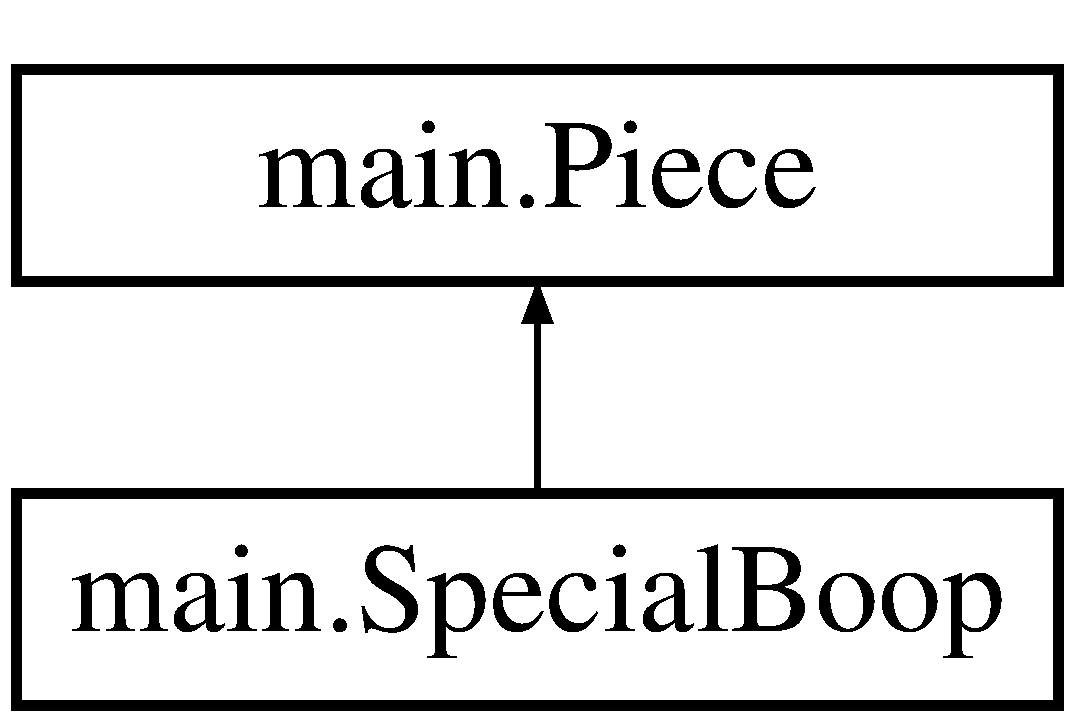
\includegraphics[height=2.000000cm]{classmain_1_1_special_boop}
\end{center}
\end{figure}
\subsection*{Public Member Functions}
\begin{DoxyCompactItemize}
\item 
\hyperlink{classmain_1_1_special_boop_aca8008b770552c3f6aaa617b8c45c463}{Special\+Boop} (int player, \hyperlink{classmain_1_1_position}{Position} position, \hyperlink{classmain_1_1_board}{Board} board)
\item 
boolean \hyperlink{classmain_1_1_special_boop_a51b7b52ee229b0a6894e76b8ac772ab6}{can\+Move\+To} (int x, int y)
\end{DoxyCompactItemize}


\subsection{Constructor \& Destructor Documentation}
\mbox{\Hypertarget{classmain_1_1_special_boop_aca8008b770552c3f6aaa617b8c45c463}\label{classmain_1_1_special_boop_aca8008b770552c3f6aaa617b8c45c463}} 
\index{main\+::\+Special\+Boop@{main\+::\+Special\+Boop}!Special\+Boop@{Special\+Boop}}
\index{Special\+Boop@{Special\+Boop}!main\+::\+Special\+Boop@{main\+::\+Special\+Boop}}
\subsubsection{\texorpdfstring{Special\+Boop()}{SpecialBoop()}}
{\footnotesize\ttfamily main.\+Special\+Boop.\+Special\+Boop (\begin{DoxyParamCaption}\item[{int}]{player,  }\item[{\hyperlink{classmain_1_1_position}{Position}}]{position,  }\item[{\hyperlink{classmain_1_1_board}{Board}}]{board }\end{DoxyParamCaption})}

Constructor for the \hyperlink{classmain_1_1_special_boop}{Special\+Boop} class 
\begin{DoxyParams}{Parameters}
{\em player} & piece player/owner \\
\hline
{\em position} & location of the piece on the board \\
\hline
{\em board} & game board \\
\hline
\end{DoxyParams}


\subsection{Member Function Documentation}
\mbox{\Hypertarget{classmain_1_1_special_boop_a51b7b52ee229b0a6894e76b8ac772ab6}\label{classmain_1_1_special_boop_a51b7b52ee229b0a6894e76b8ac772ab6}} 
\index{main\+::\+Special\+Boop@{main\+::\+Special\+Boop}!can\+Move\+To@{can\+Move\+To}}
\index{can\+Move\+To@{can\+Move\+To}!main\+::\+Special\+Boop@{main\+::\+Special\+Boop}}
\subsubsection{\texorpdfstring{can\+Move\+To()}{canMoveTo()}}
{\footnotesize\ttfamily boolean main.\+Special\+Boop.\+can\+Move\+To (\begin{DoxyParamCaption}\item[{int}]{x,  }\item[{int}]{y }\end{DoxyParamCaption})}

Function for checking if the piece can move to a specified (x,y) position on the board 
\begin{DoxyParams}{Parameters}
{\em x} & position along the x axis \\
\hline
{\em y} & position along the y axis \\
\hline
\end{DoxyParams}
\begin{DoxyReturn}{Returns}
true/false boolean whether it\textquotesingle{}s a valid move 
\end{DoxyReturn}


The documentation for this class was generated from the following file\+:\begin{DoxyCompactItemize}
\item 
src/main/Special\+Boop.\+java\end{DoxyCompactItemize}

%--- End generated contents ---

% Index
\backmatter
\newpage
\phantomsection
\clearemptydoublepage
\addcontentsline{toc}{chapter}{Index}
\printindex

\end{document}
